\documentclass[openany]{article}
\usepackage[utf8]{inputenc}
\usepackage[T1]{fontenc}

\title{Scraping Reddit, \\a Natural Language Processing Project,\\ Final Report}
\author{Bartłomiej Szymański\\
Kacper Leszczyński\\
Kamil Czerniak\\
Youssef Ibrahim\\
Igor Sałuch\\
Mike Urmich\\
Samuel Menezes}
\date{Warsaw, \\29th May 2019}


\usepackage{hyperref}
\hypersetup{
    colorlinks=true,
    linkcolor=black,
    filecolor=magenta,      
    urlcolor=blue,
    citecolor=blue
}
\usepackage{graphicx}
\usepackage{url}
\usepackage{csquotes}
\usepackage{polski}
\usepackage{english}
\setlength\parindent{0pt}
\usepackage{float}

\begin{document}
\maketitle
\newpage
\tableofcontents
\newpage

\section{Project description}

The project was pitched as a Custom Project in order to pass Natural Language Processing, a sixth semester elective course ran by Dr Agnieszka Jastrzębska at Warsaw University of Technology. \\ \\
This project combines different Data Science and Natural Language Processing principles in order to analyze different Reddit Subreddits, return tangible statistics and derive interesting conclusions about similarities and differences of different areas of the site.\\ \\
The partial goals of the program involve:
\begin{itemize}
	\item Classifying entries based on different Subreddits.
	\item Creating statistics based on entries stored in a database.
	\item Measuring what are the common factors between different Reddit Subreddits.
\end{itemize}

\begin{figure}[htb!]
    \centering
    
\includegraphics[width=\textwidth]{reddit_banner.png}
    \caption{Reddit banner}
    \label{fig:mesh1}
\end{figure}
\newpage

\section{The seven roles of the project}
There are seven members in the team, each one with a separate responsibility. Six of them have signed up for the Natural Language Processing course, while Mike Urmich was used as an external helper in the project.

\subsection{Kacper Leszczyński, Creating a database and scraping Reddit}
The first role of the program, a crucial one. Without this role nothing would be possible to achieve after that point. His responsibilities involved:
\begin{itemize}
	\item creating a database that people would be able to utilize in the later stages of the program as shown above,
	\item creating a tool that would be able to populate the database having input the Subreddit name,
	\item populating the database with at least 25 distinct Subreddits to derive interesting statistics.
\end{itemize}
\subsection{Youssef Ibrahim, Moderation, NER labelling, normalization}
His job was to cleaning up the database and opening it up for later processing by next people. His responsibilities involved:
\begin{itemize}
	\item moderating the Submissions table of the database,
	\item lemmatization of the sentences, removing markdown,
	\item creating a list of NER attributes for Submissions and Comments and inserting it into the database.
\end{itemize}
\subsection{Kamil Czerniak, finding the most common words, creating statistics}
The first of the asynchronously assigned jobs, his goal was to operate on single words on each of the Comments and aggregating them in statistics that would later be turned into report sections. His responsibilities involved:
\begin{itemize}
	\item creating .csv files with the most common words based on Subreddits,
	\item running a classifier for positive and negative sentiments of different Subreddits,
	\item creating .csv files that could later be used to create data tables.
\end{itemize}

\subsection{Samuel Menezes, creating and optimizing database classifiers}
The goal of this job was to make it so that, based on the input data from a console window, information regarding various statistics of Submissions and Comments tables would be displayed. His responsibilities involved:
\begin{itemize}
	\item creating classifiers that would allow to get moderately reliable information about the post/comment based on the data in the database,
	\item optimizing classifiers by removing unnecessary data,
	\item arranging statistics data into sensible data tables.
\end{itemize}

\subsection{Igor Sałuch, creating an interface for interacting with classifiers}
Having received the previous classifiers, the goal of the person is was create a versatile and user-friendly graphical interface for interacting with classifiers. His responsibilities involved:
\begin{itemize}
	\item creating a user-friendly graphical interface based on the classifiers and data tables obtained before,
	\item making sure it was possible to, depending on different input data, get different statistics regarding the posts,
	\item making the return data of the application be approximate and not equal to the result to avoid introducing uncertainty biases.
\end{itemize}

\subsection{Mike Urmich, finding correlations between Subreddits}
Looking at the database and statistics created by Kamil, finding interesting data across different Subreddits. His responsibilities involved:
\begin{itemize}
	\item grouping Subreddits based on different criteria,
	\item finding interesting statistics among the CSV files,
	\item writing a part of the report with found statistics.
\end{itemize}

\subsection{Bartłomiej Szymański, coordinating, scripting charts and report}
The final role, combining the work of all other team members, fixing their missteps, deriving conclusions and making charts for each of the statistics. His responsibilities involved:
\begin{itemize}
	\item coordinating the work of everyone involved in the project,
	\item creating classifiers, creating charts to statistics,
	\item writing a huge part of the report.
\end{itemize}

\section{Technical details}
Every observation in this document follows a snapshot of Reddit Subreddits scraped between March 16th and 19th, 2019. \\ \\
Every Subreddit that was considered has been scraped according to at most 1,000 all-time highest rated posts, with 100,000 comments and the end of a given Submission being a limit for each of the Subreddits before moving onto the next one (the theoretical maximal amount of Comments from one Subreddit being 101,999).\\ \\
The scraping algorithm has been set to not scrape Submissions that have more than 2,000 Comments to avoid a scenario where 7-8 Submissions would be enough to populate the database for a given Subreddit with Subreddits such as /r/iama or /r/news. Those Submissions still get added to a Submission table, just their Comments do not get added to the Comments table.\\ \\
The database to which all the Comments have been scraped is available on Google Drive. (\href{https://drive.google.com/file/d/1eVMN0cTHSuY3mnnkM8_UgkqlXlvftJlg/view?usp=sharing}{Raw database}, \href{https://drive.google.com/file/d/1qpjm8K_cQ629oUhFt389x_uQDdVuk-E2/view?usp=sharing}{Moderated database}). \\ \\
There are three tables in it, one for Subreddits and their names, one for Submissions and one for Comments. The tables follow \href{https://github.com/scrapingredditboys/ScrapingRedditNaturalLanguageProcessingWUT2019/blob/master/reddit-collector/tables.sql}{this structure}.\\ \\
The list of 55 Subreddits scraped to the database looks as follows:
\begin{quote}
spacex,	KerbalSpaceProgram,	Bitcoin,	pcmasterrace,	Showerthoughts,	outside,	dankmemes,	wholesomememes,	2meirl4meirl,	WritingPrompts,	tifu,	news,	nottheonion,	4chan,	Music,	IAmA,	math,	itookapicture,	learnprogramming,	gaming,	movies,	mylittlepony,	anime,	sports,	gonewild,	europe,	apple,	Android,	ATBGE,	depression,	disneyvacation,	mildlyinteresting,	interestingasfuck,	mildlyinfuriating,	worldnews,	furry\_irl,	talesfromtechsupport,	TalesFromRetail,	nosleep,	hmmm,	NintendoSwitch,	smashbros,	nostalgia,	Drugs,	dankchristianmemes,	aww,	polandball,	WTF,	FortNiteBR,	GetMotivated,	Fitness,	Drama,	netflix,	PewdiepieSubmissions,	Minecraft
\end{quote}


\subsection{Verifying if Subreddits are good targets for scraping}

A \href{https://github.com/scrapingredditboys/ScrapingRedditNaturalLanguageProcessingWUT2019/blob/master/reddit-collector/validator.py}{special tool} has been developed by Kacper Leszczyński to verify if a given Subreddit is a good target for scraping operation. \\ \\
It takes Subreddit names as input parameters and based on our applied criteria (API can return up to 1,000 top rated posts of all time, the amount of Comments in a Submission cannot exceed 2,000) finds if it's possible to obtain 100,000 Comments.

\begin{figure}[htb!]
    \centering
    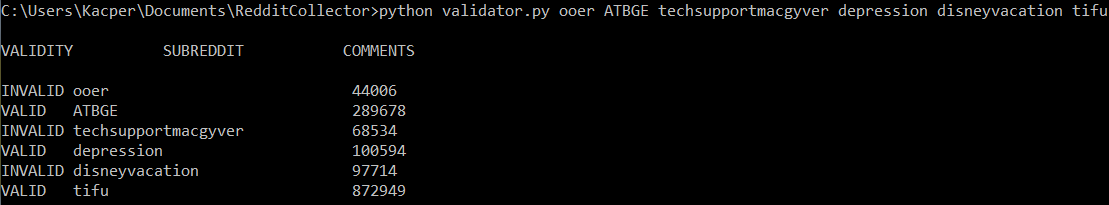
\includegraphics[width=\textwidth]{validator.png}
    \caption{the Subreddit validator in action}
    \label{fig:mesh1}
\end{figure}

Sixteen Subreddits on the list that have not met 100,000 Comments have been added to the list regardless. 11 of them have more than 90,000 Comments though.

\subsection{Scraping the database}
Upon verifying that a Subreddit was a good target for scraping, the \href{https://github.com/scrapingredditboys/ScrapingRedditNaturalLanguageProcessingWUT2019/tree/master/reddit-collector}{following script by Kacper Leszczyński} was ran on 55 different Subreddits, mentioned above. Because of Reddit API limitations, one query could only be ran every 2 seconds, which made the script's execution take a couple of days. Each next row was appended to a database in a PostgreSQL format.\\ \\
The database contains 3 tables, one containing information on Subreddit names, one containing information on Submission names and threads that contain Comments, and one containing over 5 million Comments.

\subsection{Cleaning up the database}
Youssef Ibrahim went through the initial database and applied a process of database normalization, through iterating through every one of the over 5 million Comments in the database, he faced a number of challenges:
\begin{itemize}
    \item To remove stop words from sentences or not? Ultimately we have decided to remove all stop words that NLTK library considered to be stop words\cite{stopwords}. Thanks to that, database size decreased dramatically.
    \item Stemming, or Lemmatization? Ultimately, lemmatization was chosen as the final method of normalizing the database.
    \item Recognizing more Named Entities in the database, because of how chaotic internet communication can be, sometimes words such as "Space X" will not be recognized as a Named Entity, for that reason some words needed to be manually added to a Named Entity Recognition database
    \item How to remove punctuation and special characters and keep them in other special cases? For this purpose both Regex and NLTK library have been used. Unfortunately, this led to a problem where the words such as "we'll" and "they'll" have been split into two separate words.
    \item The size of a database. Parsing the comments took a weekend running 10 different instances of Google Colab simultaneously and the table has been connected afterwards.
\end{itemize}
Due to the process of cleaning up, four Subreddits' data has been lost: /r/KerbalSpaceProgram, /r/Netflix, /r/PewdiepieSubmissions and /r/Minecraft.

\subsection{Arranging the data in data tables}
\label{sec:datatables}
Based on raw data extracted from the database by Kamil Czerniak, we were able to arrange some of data in data tables that could later be used to run statistics on those tables. This duty was performed by Samuel Menezes. Our final project contains seven distinct data tables, available in \href{https://drive.google.com/drive/folders/1ROxIWmS5nnnhzwUUQuyAWV5oK8KLdnb9}{this} directory. The Data Tables involve:
\begin{itemize}
    \item \textit{Calculation of Mean Sentiments of Comments} tested against an IMDb review labeled database \cite{sentimentanalysis}, where the reviews were classified based on whether they were positive or negative. \\
    \textit{Warning}, due to the way the data was provided in that table, negative values are attributed to positive sentiment, and positive values to negative sentiment of the messages.
    \item \textit{Karma of Comments based on lengths of Comments in characters}, where a character count was added up and an average amount of letters has been calculated.
    \item \textit{Positive (and Negative) Sentiments of Submissions based on upvote ratio}, based on what was the amount of upvotes in comparison to downvotes, we can determine if the posts were positive or negative, tested against the same database.
    \item \textit{Number of Comments based on hour (and weekdays and hours)}, depending on the time of the day and the day of the week, how many Comments have been posted.
    \item \textit{Karma of Comments based on hour of posting}, depending on the time of the day and the day of the week, how much karma have comments obtained on average.
\end{itemize}
Thanks to those data tables, it was much easier to create statistics in the later part of the database.
\subsection{Creating classifiers}
Our final database involves three classifiers, all three prepared from different sources. The first one has been provided by Samuel Menezes, the remaining two by Bartłomiej Szymański. All three classifiers are located in  \href{https://drive.google.com/drive/folders/1lTxPU9afFa5V2qXWcALFKBRBgVuEu87F}{this} directory.
The responsibilities of classifiers involve:
\begin{itemize}
    \item \textit{Average Word Usage Classifier}, words that are distinct to one Subreddit are posted as rows in this classifier with coefficients describing the odds of how likely is the word to come out of this Subreddit. \\ \\
    Optimization: removing words whose popularity in every Subreddit was less than 5.9\%. If a word has been used in at least one Subreddit for more than 5.9\% compared to the rest of the uses in the database, it has been added as a row to the Classifier.
    \item \textit{Emotion Classifier}, attributing certain values divided into Valence, Arousal and Dominance coefficients from a Saif M. Mohammad dataset\cite{emotions}. \\ \\
    Optimization: removing words from the dataset that have not been mentioned in our database, leading to a reduced amount of rows.
    \item \textit{Topics Classifier}, listing what topics are connected to each of the words, based on WordNet database \cite{wordnet}. \\ \\
    Optimization: just as above, removing words from the dataset that have not been mentioned in our database, leading to a reduced amount of rows.
\end{itemize}
\subsection{Displaying data tables and classifying sentences to categories}
An interface for interacting with data tables and classifying sentences has been created by Igor Sałuch, this is the most user-friendly method of interacting with data tables and getting information on what emotions, topics and Subreddits are the sentences typed into the window from.\\ \\
The application loads up .csv files from the previous two sections, and based on that returns sentences in human readable format about .csv file parameters.
There are 5 sections in the application dedicated to reading data tables, the same one as in the  \hyperref[sec:datatables]{data table section}. Sections most often take Subreddit names as input parameters and depending on a category, either a weekday/hour of a week, upvote ratio or the comment length. A sample output of the program is shown in the figure below. 

\begin{figure}[H]
    \centering
    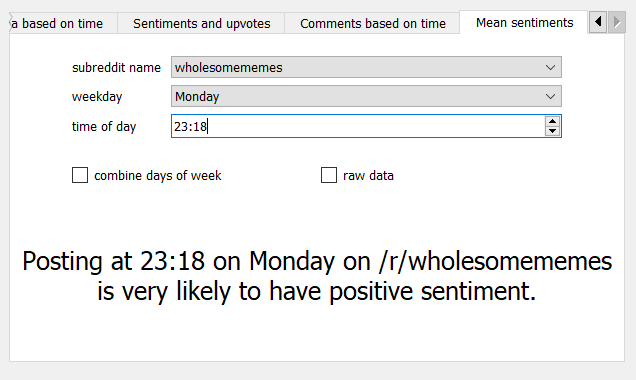
\includegraphics[width=\textwidth]{Data_Table_Interaction.png}
    \caption{Sample screenshot of investigating Mean Sentiments of messages in the data table visualization tool}
    \label{fig:mesh1}
\end{figure}

There is one additional section devoted to classification of sentences input into the program with a lengthy input box. Upon pressing a button, words are read from the input box and attributed three different coefficients: Subreddit the message is most likely to be from, the emotion it is most likely to possess and a topic that is the most prevalent in the message.

\begin{figure}[H]
    \centering
    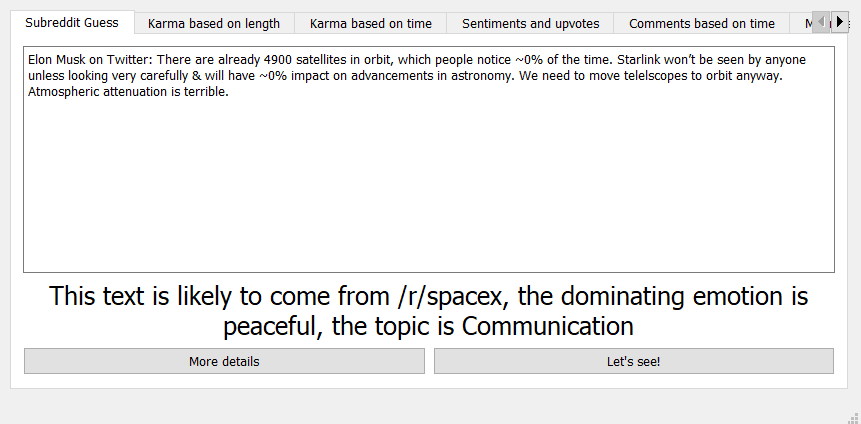
\includegraphics[width=\textwidth]{Classifier_Interaction.png}
    \caption{Sample screenshot of working with the Classification Window}
    \label{fig:mesh1}
\end{figure}

\subsection{Finding n-grams in the database}
Another utility has been developed by Kacper Leszczyński, which takes a substring and returns n-grams of chunks of words in a text by connecting to the database. The tool supports multiple n-lengths, the substring can be of any arbitrary length and has been used to create a later part of the report.\\ \\
Initially the script ran very slow, but through the process of setting a server-side cursor upon the database to which the script was connected to, the script sped up tremendously.

\subsection{Scripts for preparing charts}
Utilizing data created by other people and custom-created .csv files, a list of scripts was created in Python and R Studio by Bartłomiej Szymański and Mike Urmich in order to create charts present in this report in here.\\ \\
Every chart has been prepared in PDF vector format with the help of Microsoft Excel by importing .csv files and adjusting some coefficients of the charts.\\ \\
Since PDF format is vectorized, it is possible to zoom up into the charts indefinitely.

\newpage
\section{Statistics}
\subsection{General data}
The final database contains 5,128,536 Comments and 19,203 Submissions from 55 different Subreddits. /r/intetestingasfuck has the most Comments in the entire database sitting at 101,721, 11 Subreddits gathered less than 100,000 Comments, while still being in an accepting range and 4 Subreddits have had their data lost in the process of Normalization.\\ \\
\begin{figure}[H]
    \centering
    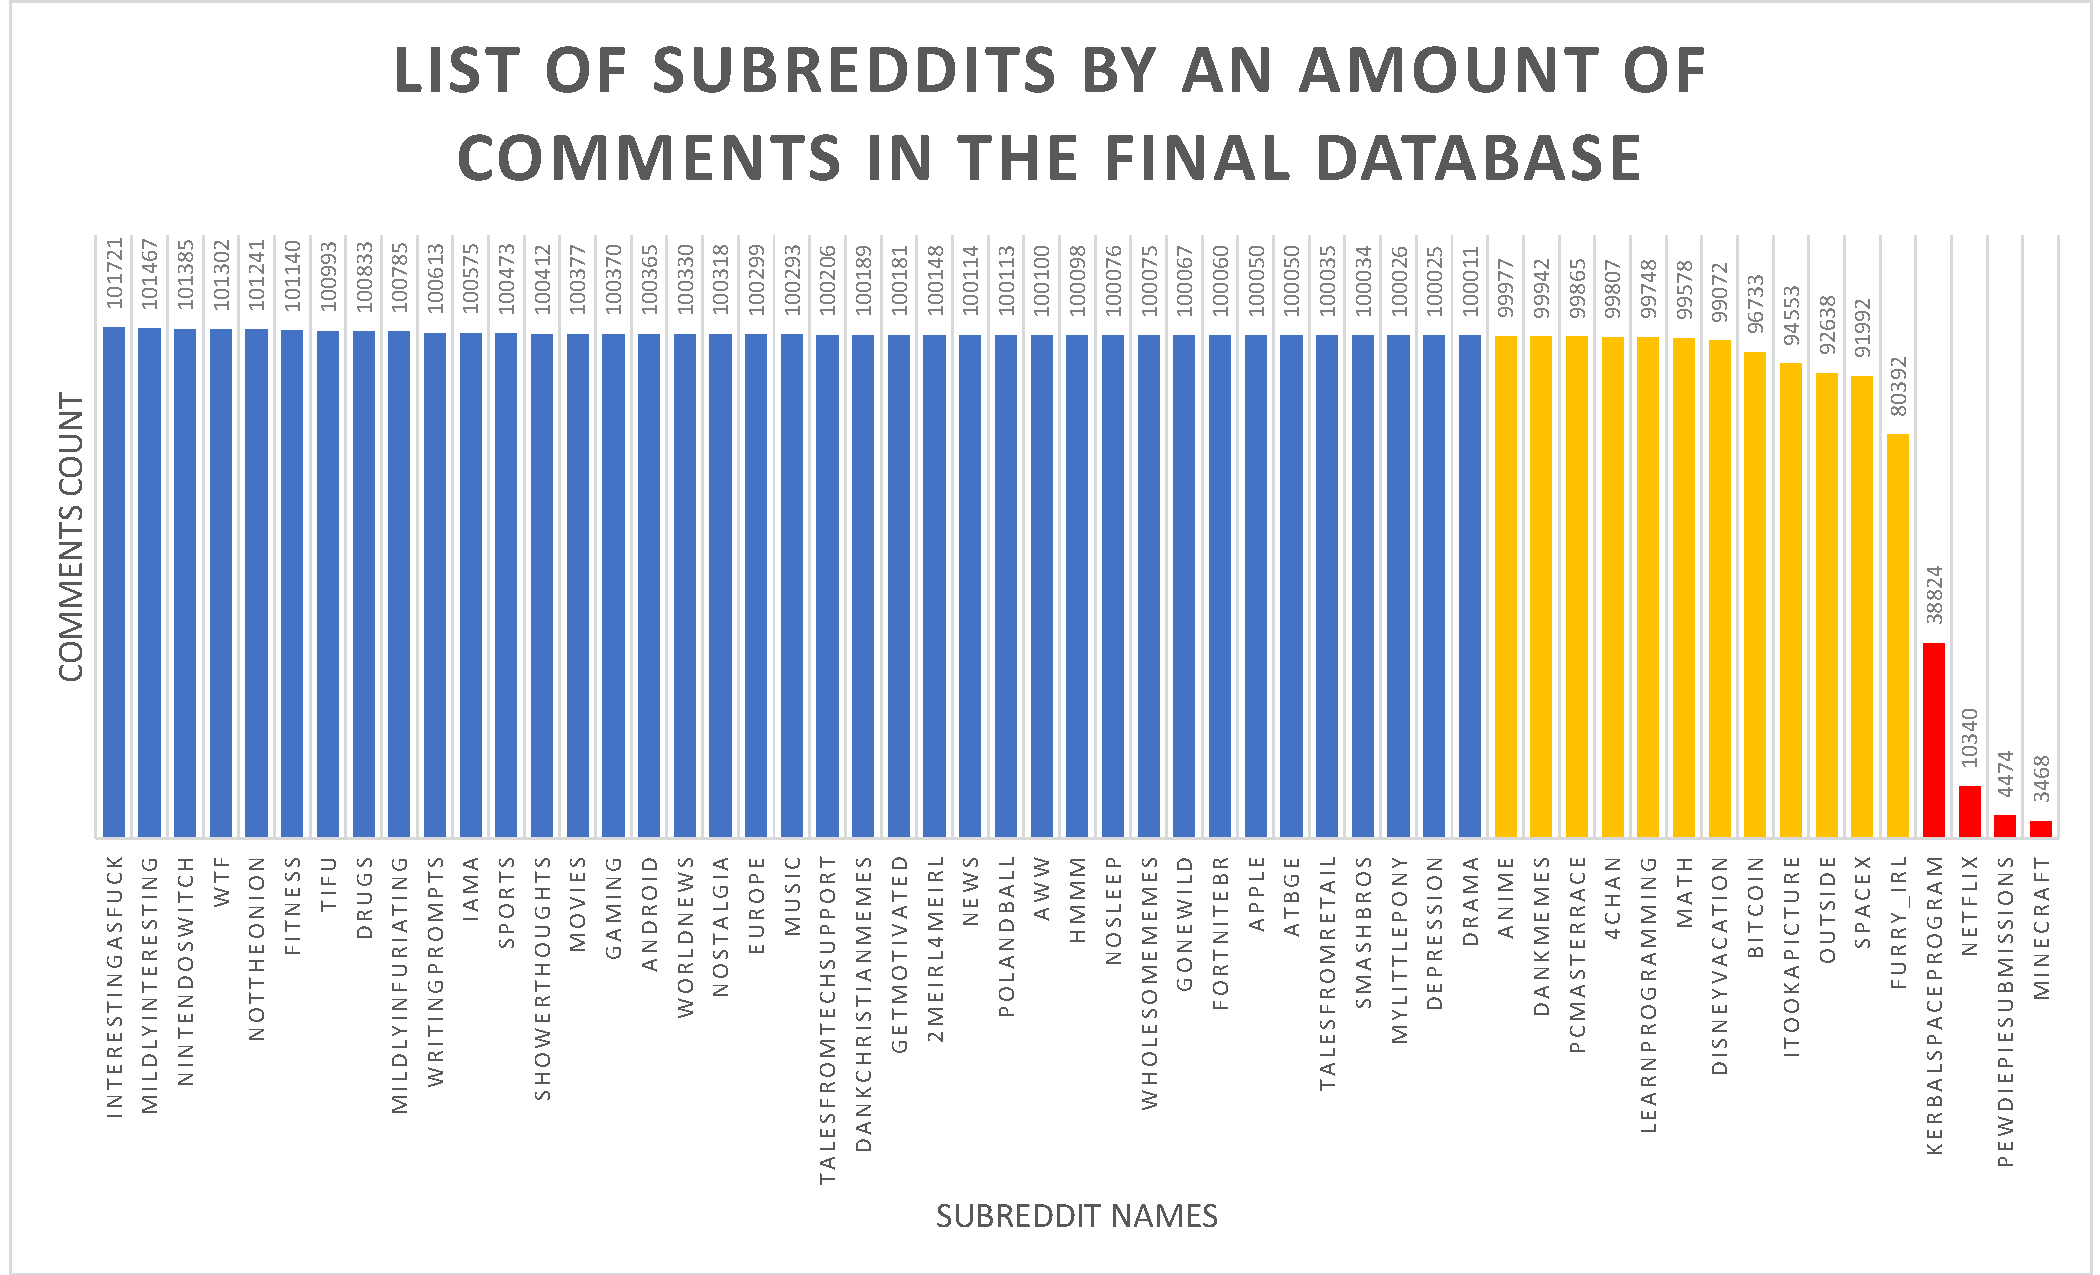
\includegraphics[width=\textwidth]{subredditsbywords.pdf}
    \caption{List of Subreddits by comment count in the final database}
    \label{fig:mesh1}
\end{figure}
The final database contains 44,635 unique words, out of which 22,637 are English words according to the Python nltk library statistics. There are 1,290,498 unique commenters and 14,360 unique submission posters.
The moderated database without compression weighs 1.42 GB when compressed the size is down to 382 MB.

\subsection{Most common posting times}
Every timestamp in the database is stored with a UTC timestamp, so all the hours in the following section are mentioned with a UTC time zone in mind.
\subsubsection{Most common posting hours of a day}
Because Reddit is an American site, hours between 4PM and 4AM are the most common hours for posting when considering UTC zone, which translates to hours from 11AM to 11PM Pacific Daylight Time or 2PM to 2AM Eastern Daylight Time.\\ \\
The single most posted hour in the database that we have is 8PM UTC at 283,073 Comments.
\begin{figure}[H]
    \centering
    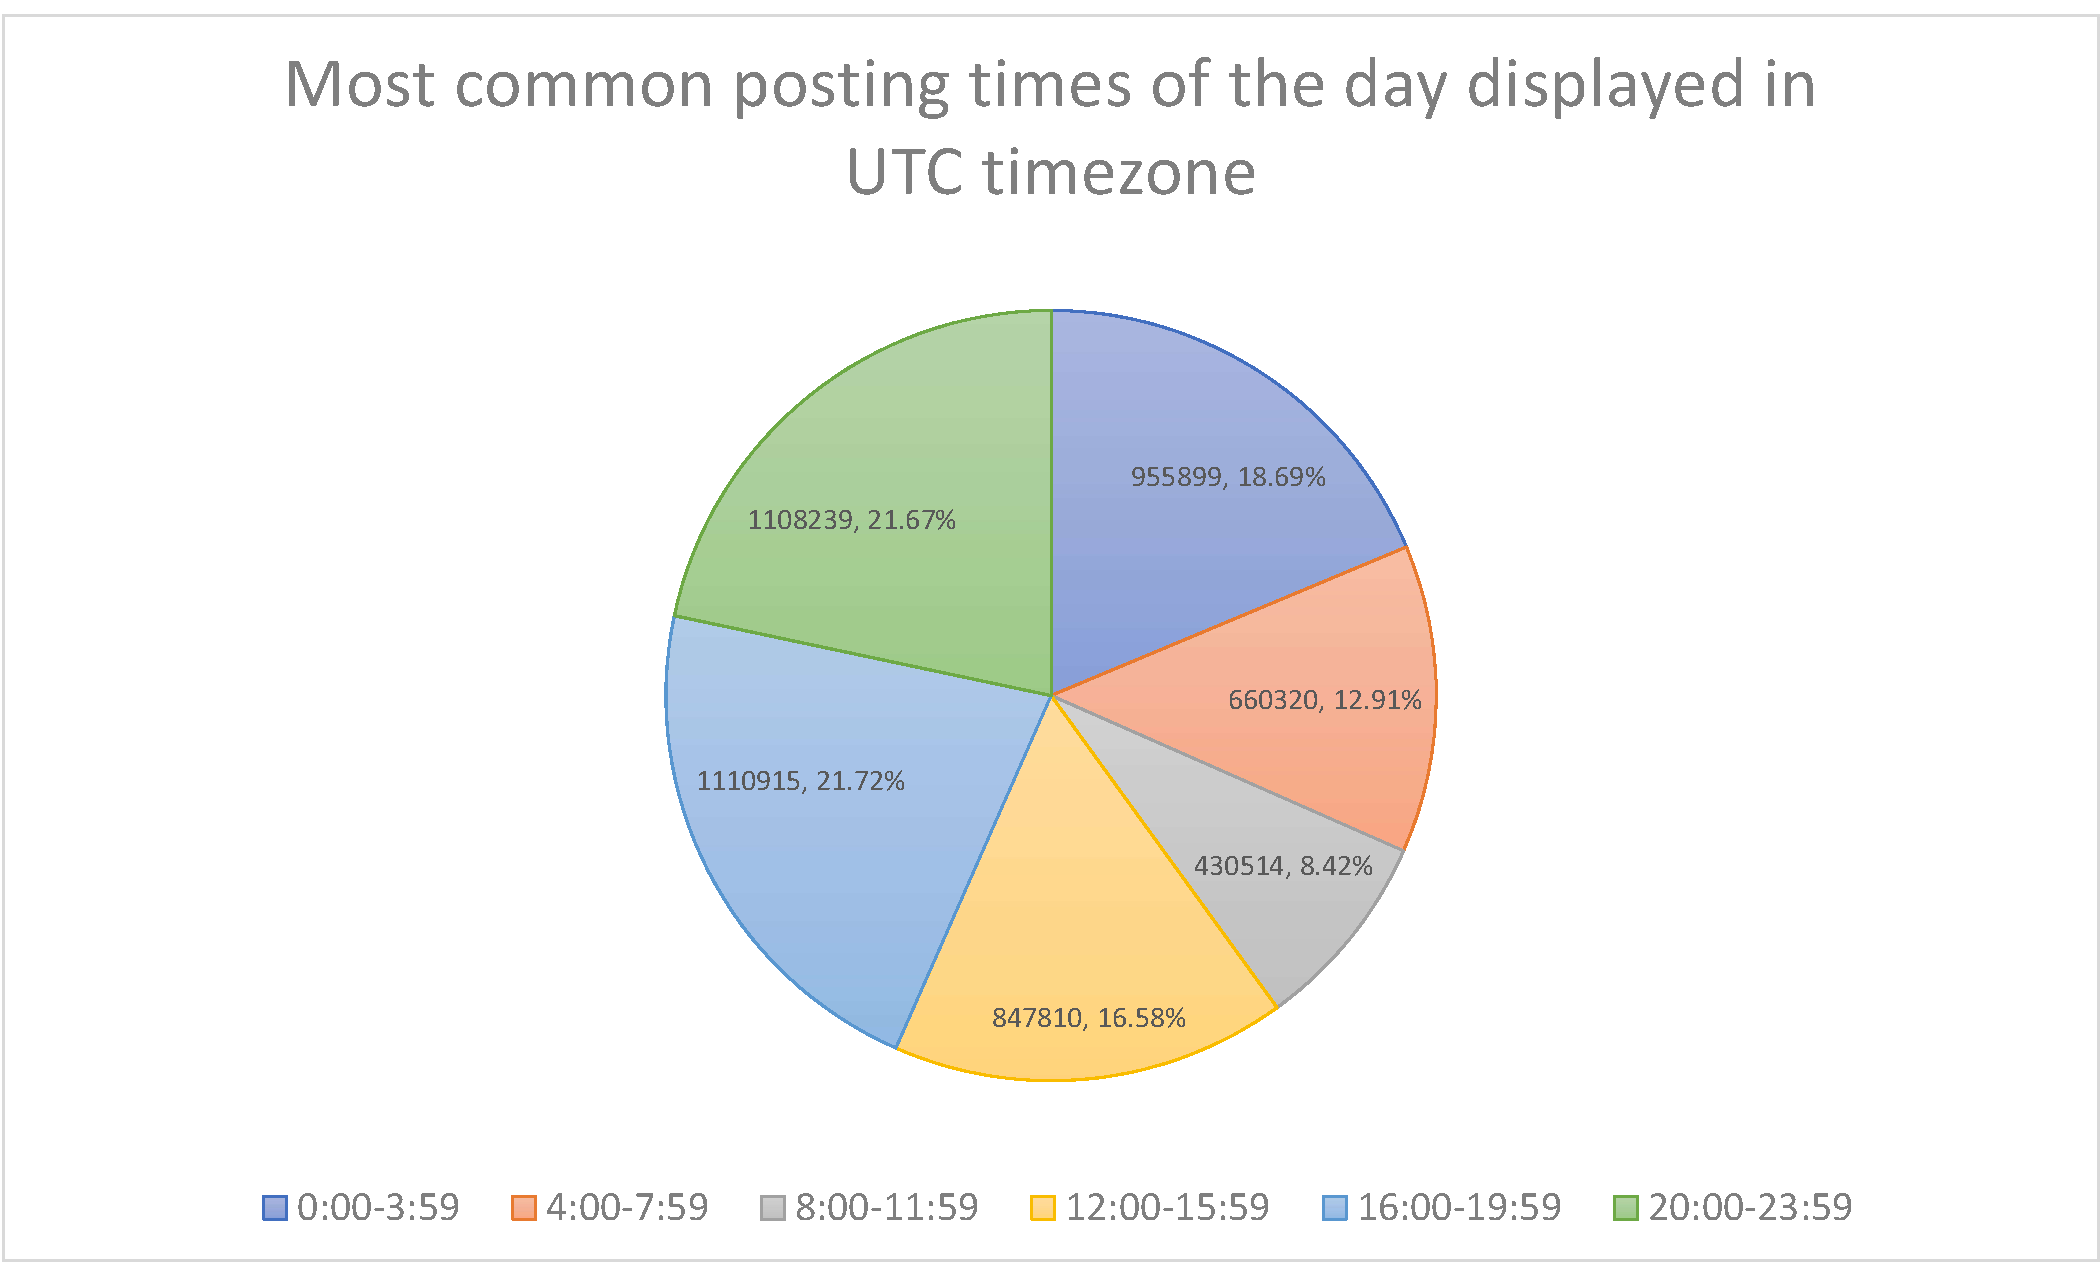
\includegraphics[width=\textwidth]{postingtimes.pdf}
    \caption{A depiction of the most common posting times of the day on Reddit based on Comments from the database in UTC time zone}
    \label{fig:mesh1}
\end{figure}

\subsubsection{Most common posting days of the week}
As it turns out, the most popular day of the week for posting is Wednesday, followed closely by Thursday and Friday. Weekend days see the least posts on the platform, but the split between various days of the week is mostly similar. \\ \\
The reason for weekdays being more popular than weekend days can be attributed to the fact people most often browse Reddit while at work, but they spend their weekends off doing other, not work and not online related activities.
\begin{figure}[H]
    \centering
    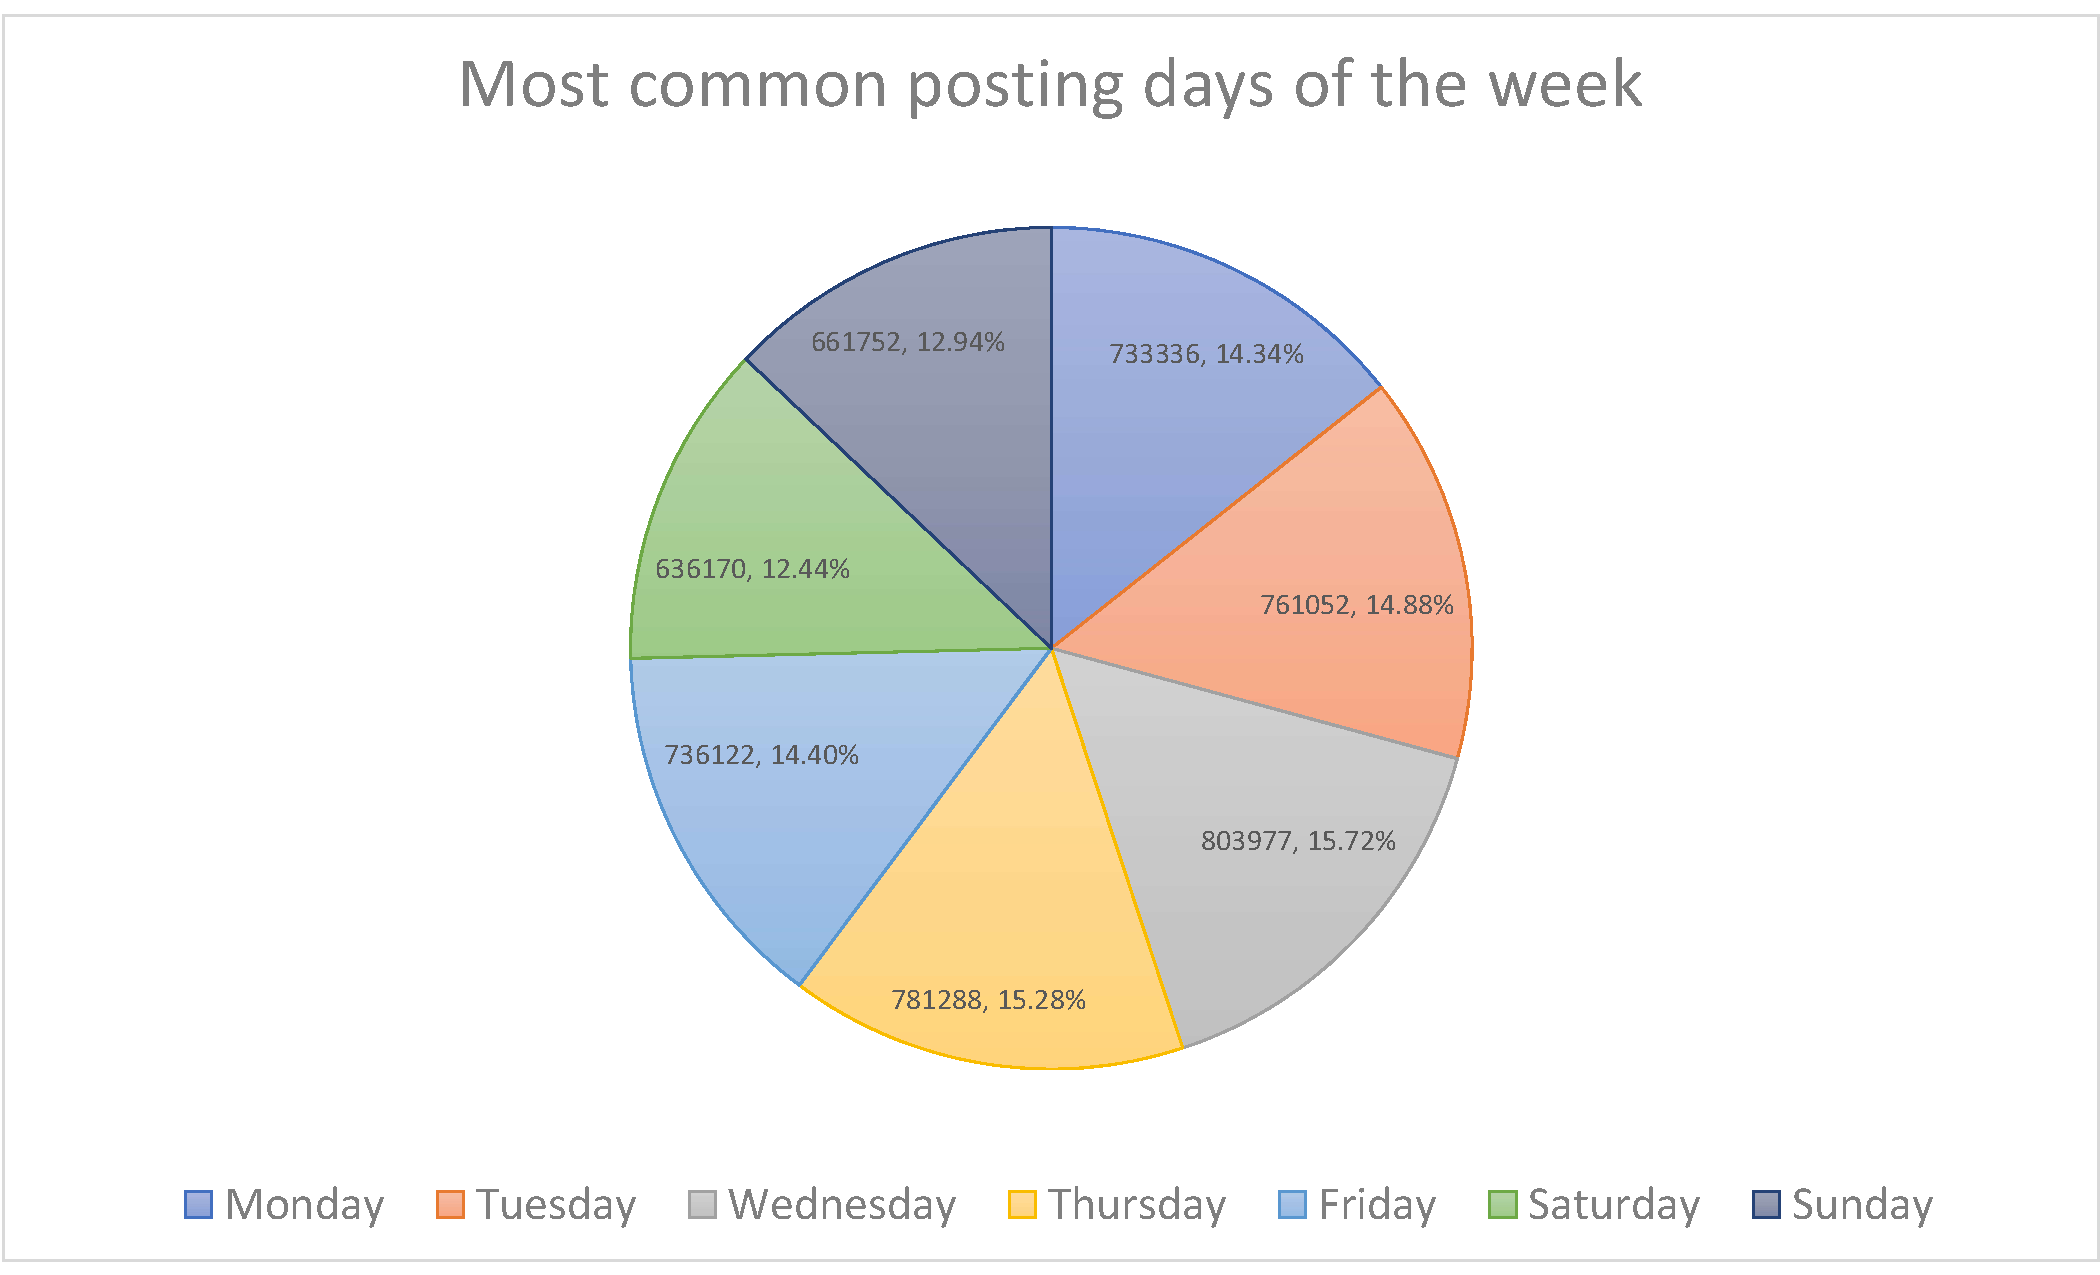
\includegraphics[width=\textwidth]{postingdays.pdf}
    \caption{A depiction of the most common posting days stored in our database}
    \label{fig:mesh1}
\end{figure}


\subsection{Most popular posters}
The most common commenters in the database are, unsurprisingly, bots. Three of the top positions are held by u/Automoderator, u/pewdsvstseries\_bot and u/furbot\_. There are only 31 commenters who have written more than 500 Comments and a huge chunk of it consists of bots. The most active non-bot commenter was \href{https://www.reddit.com/user/catoticneutral/comments/}{u/CatoticNeutral} at 1193 Comments in the database. \\ \\
In the Submission posting department, no user has posted more than 57 Submissions that made their way to the database with \href{https://www.reddit.com/user/maxwellhill}{u/Maxwellhill} having posted that many Submissions.
\begin{figure}[H]
    \centering
    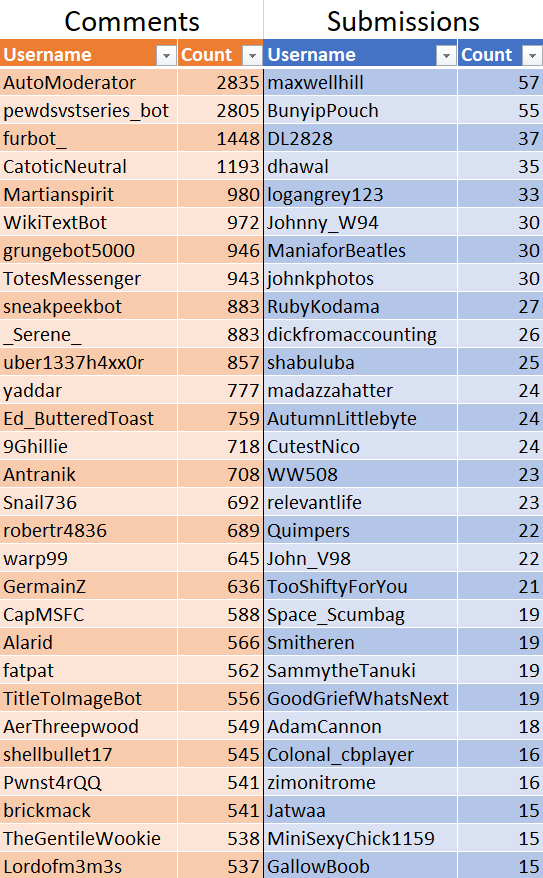
\includegraphics[width=0.6\textwidth]{Posters.png}
    \caption{List of users that have posted the most Comments and Submissions that made their way to the final database}
    \label{fig:mesh1}
\end{figure}

\subsection{Most popular words}
\subsubsection{In the whole database}
After removing stop words and words that do not belong to English Dictionary, it turns out that the most popular words in the database are verbs. The first most commonly used noun shows up on the third most popular position, the word "one". The word "one" has been used 446,929 times, the word "two" 82,903 times, the word "three" brings the number down to 23,260
times, "four" down to 9,636 times.
\begin{figure}[H]
    \centering
    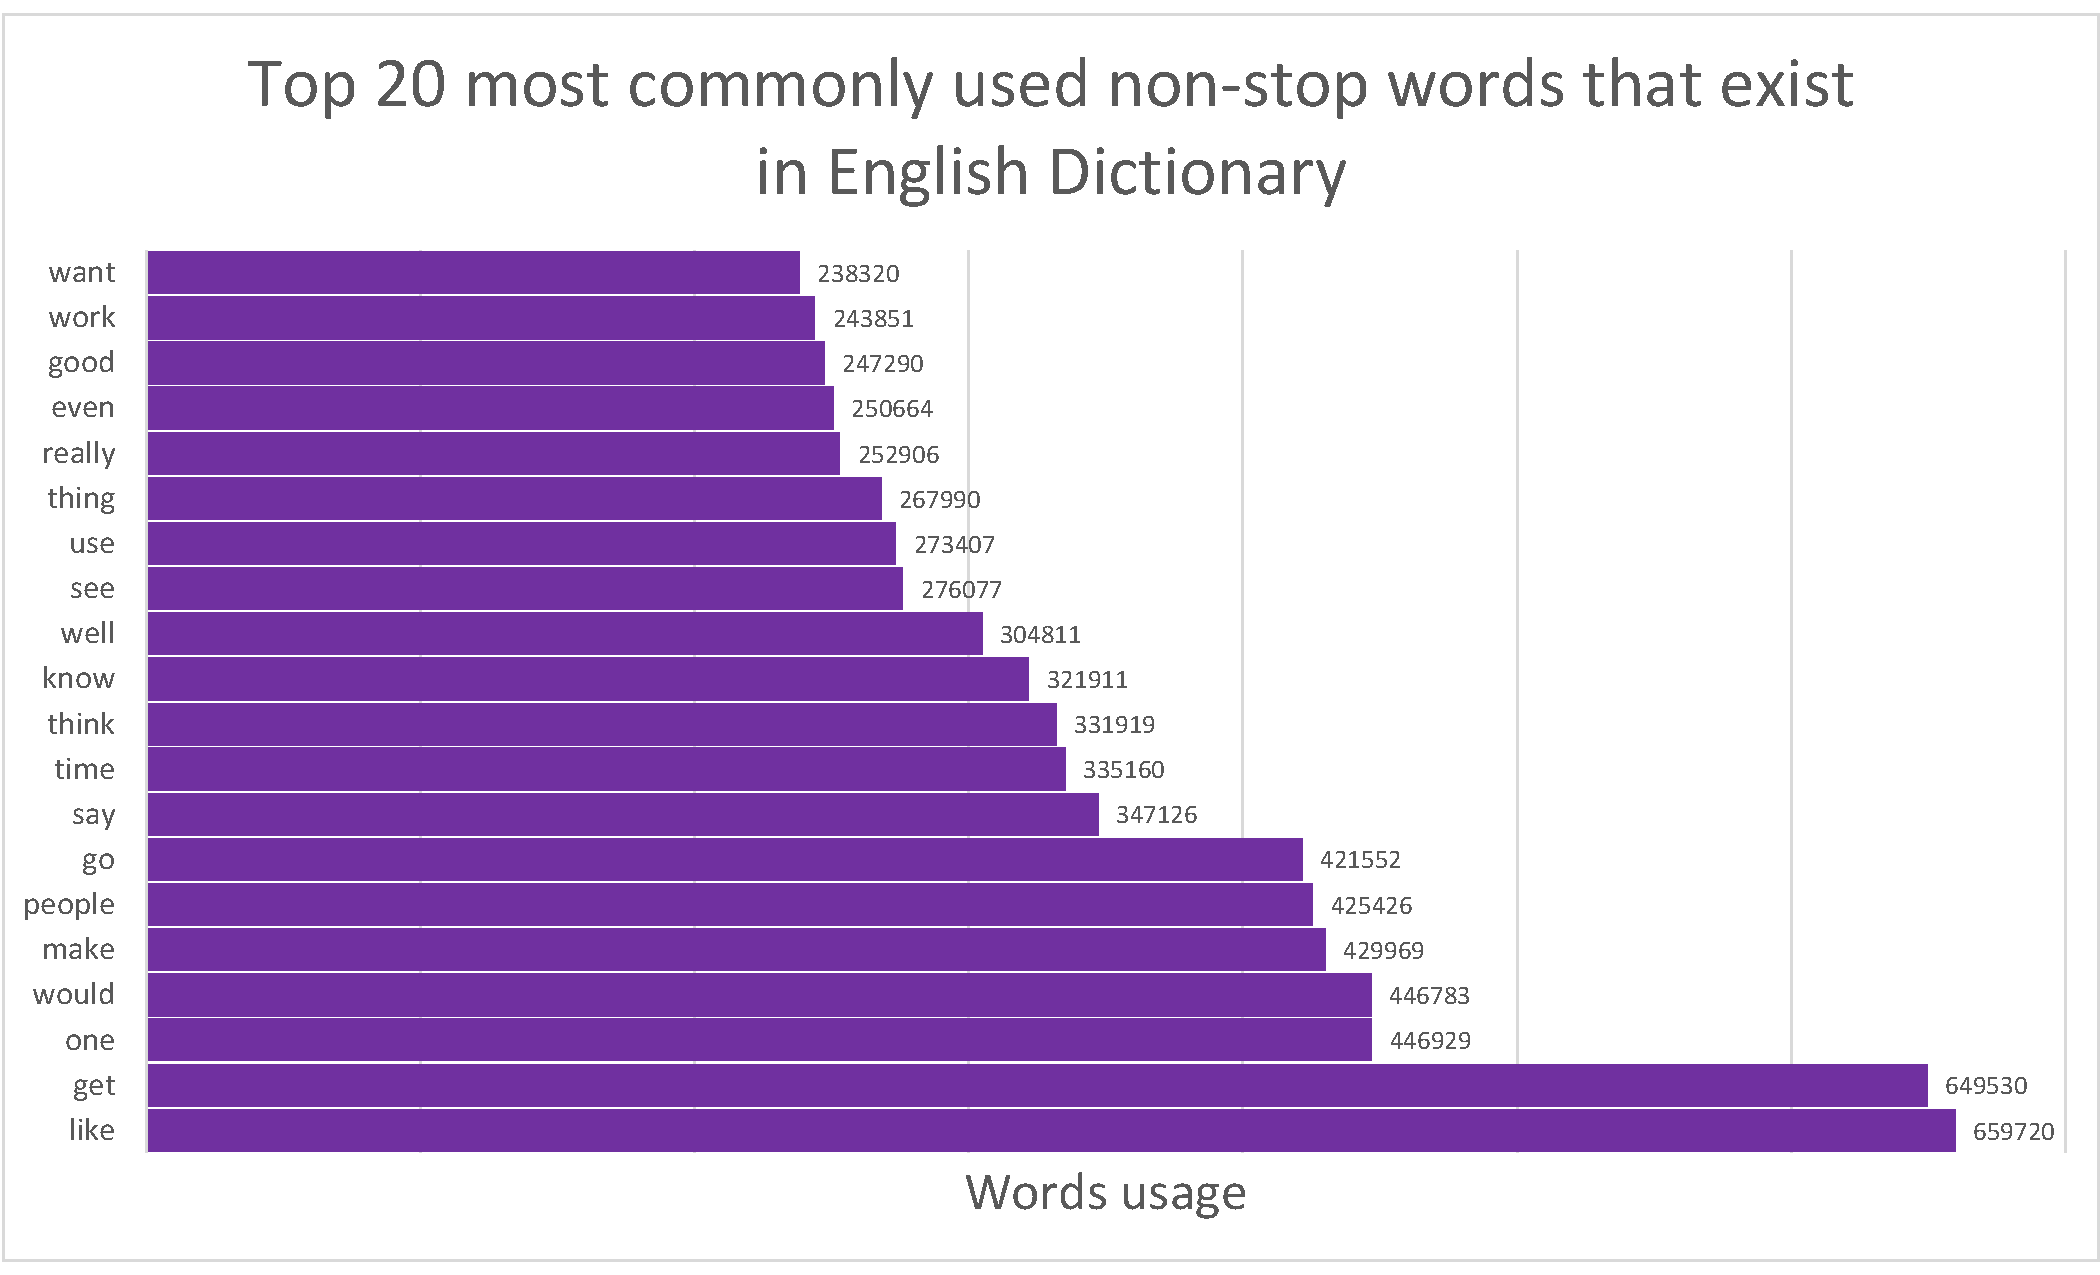
\includegraphics[width=\textwidth]{topusedwords.pdf}
    \caption{A depiction of the top 20 most posted words in the database}
    \label{fig:mesh1}
\end{figure}

\subsubsection{Very popular in one of the Subreddits}
To perform this experiment, the following conditions were considered:
\begin{itemize}
    \item A word would be mentioned in 4 Subreddits at most
    \item A word would be mentioned in one of the Subreddits at least 80\% of the time compared to the other Subreddits
    \item A word would not come from /r/PewdiepieSubmissions Subreddit because that Subreddit was incorrectly parsed
\end{itemize}
The results of the experiment were interesting. In 500 first words, the most words came from /r/mylittlepony Subreddit, with 126 distinct words. \\ \\
Most of the words found with that criteria were names of emoticons exclusive to this Subreddit, which sheds interesting light on this Community being distinct from the others, as not many other Subreddits even have their own emoticons to begin with.

\begin{figure}[H]
    \centering
    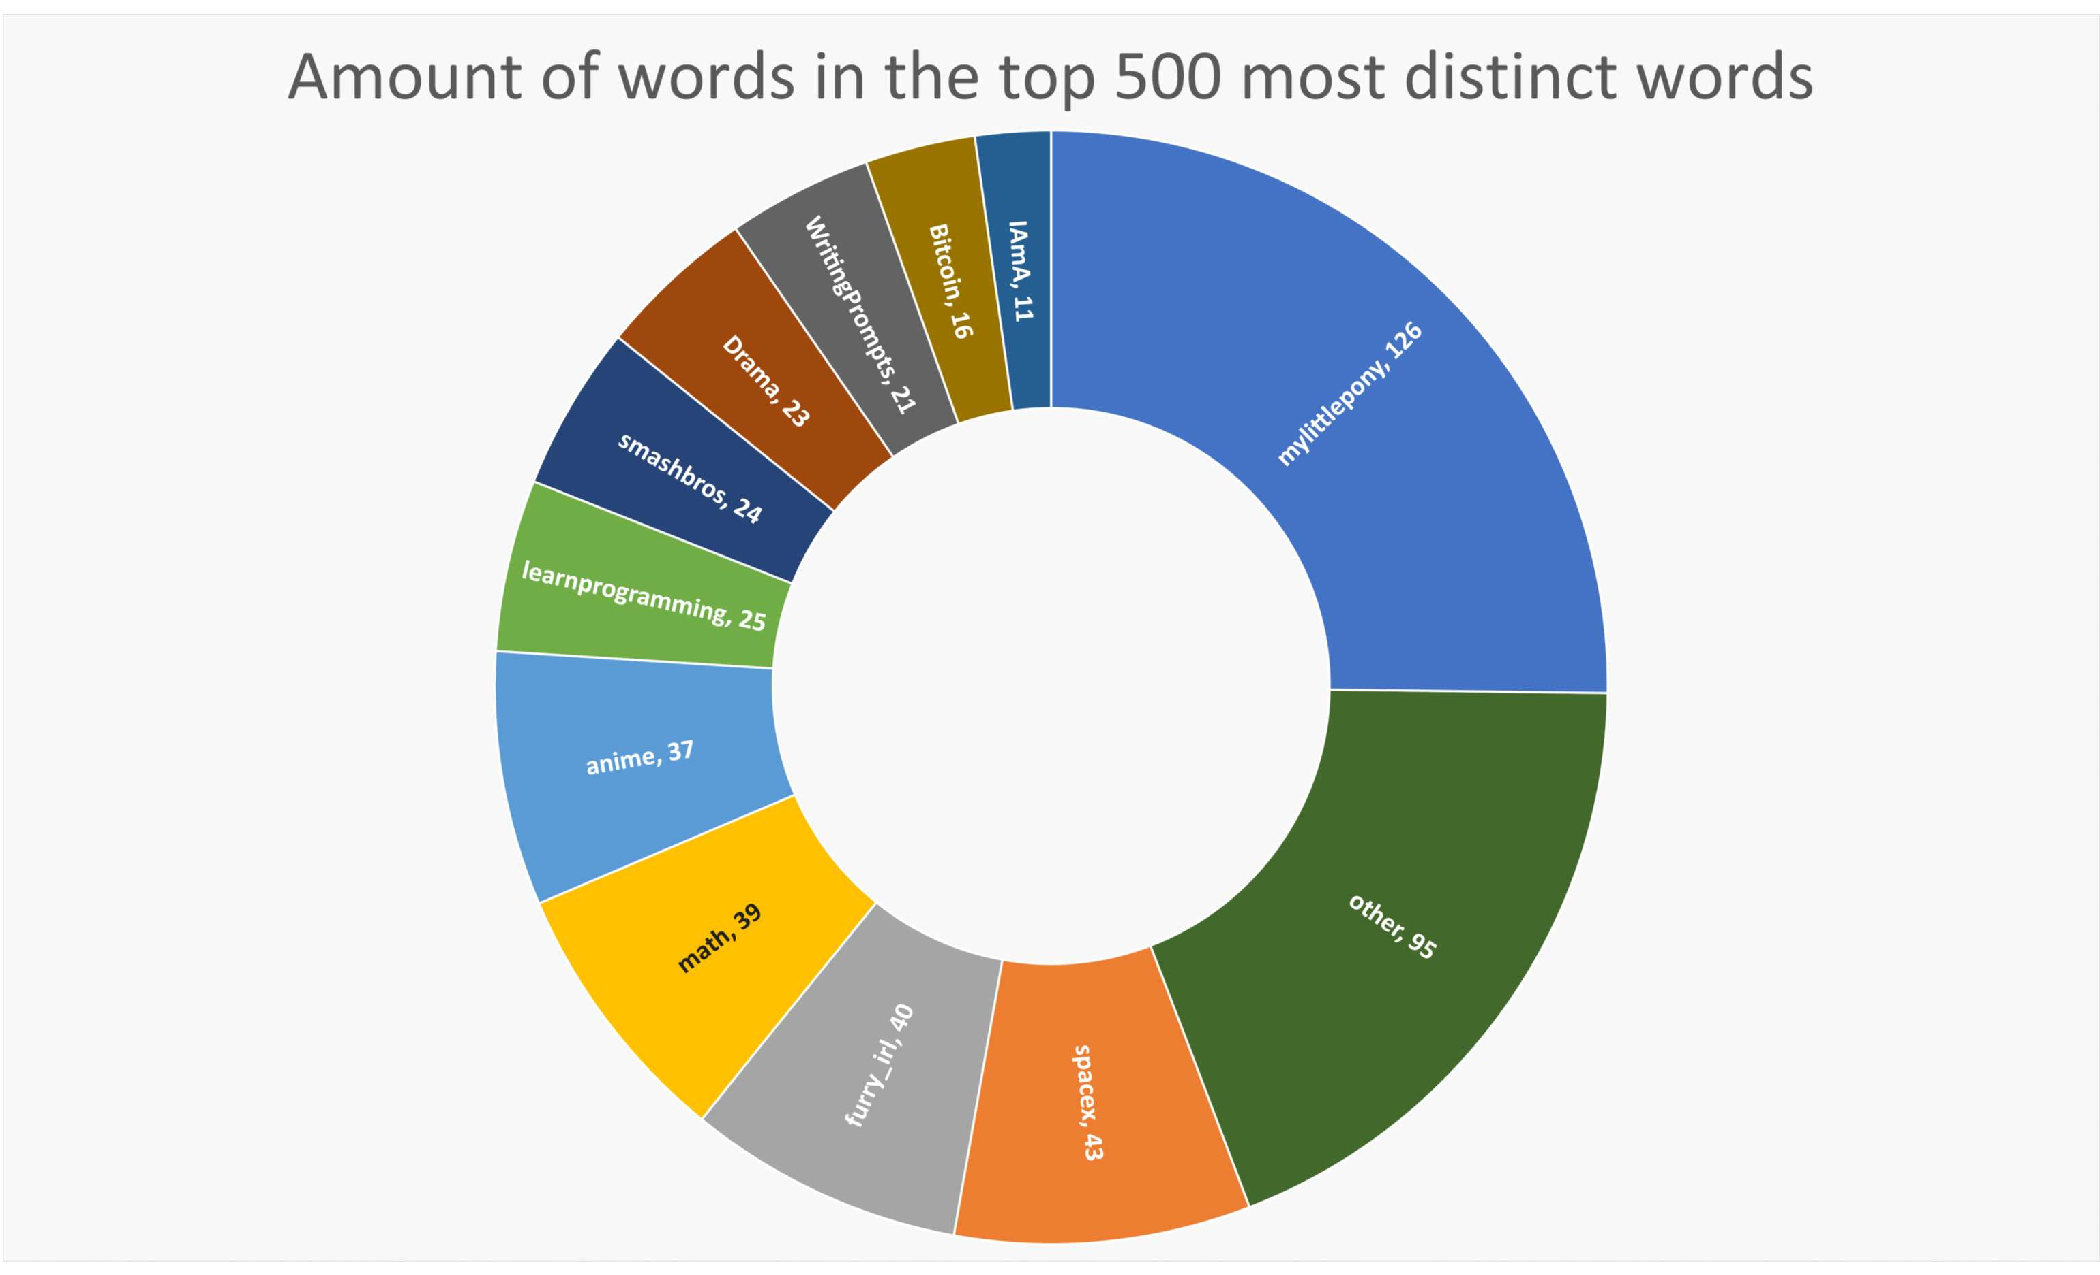
\includegraphics[width=\textwidth]{top500distinctwords.pdf}
    \caption{The Subreddit distribution of 500 most popular distinct words using criteria specified above}
    \label{fig:mesh1}
\end{figure}
Out of those 500 words, the most common ones involve:
\begin{itemize}
    \item b18, a sexual emoticon popular in 2011-2013 on /r/mylittlepony Subreddit,
    \item pixel871, a man mostly known in the /r/furry\_irl Subreddit for having, \href{https://np.reddit.com/r/delusionalartists/comments/8y1mfe/furbuy_is_a_goldmine_500_for_this_kangaroo/e27nibu/?context=1}{posted an explanation} of what a "fursona" is
    \item plup, a Smash Bros Player popular with fans for his explosive personality,
    \item cs50, a \href{https://www.edx.org/course/cs50s-introduction-to-computer-science}{course of introduction} to Computer Science,
    \item sakuta, given name of Sakuta Azusagawa, the protagonist of anime series called \textit{Seishun Buta Yarou wa Bunny Girl Senpai no Yume wo Minai}, which was popular in mid-2018,
    \item kerbin, the home planet of Kerbals in Kerbal Space Program.
\end{itemize}

\begin{figure}[H]
    \centering
    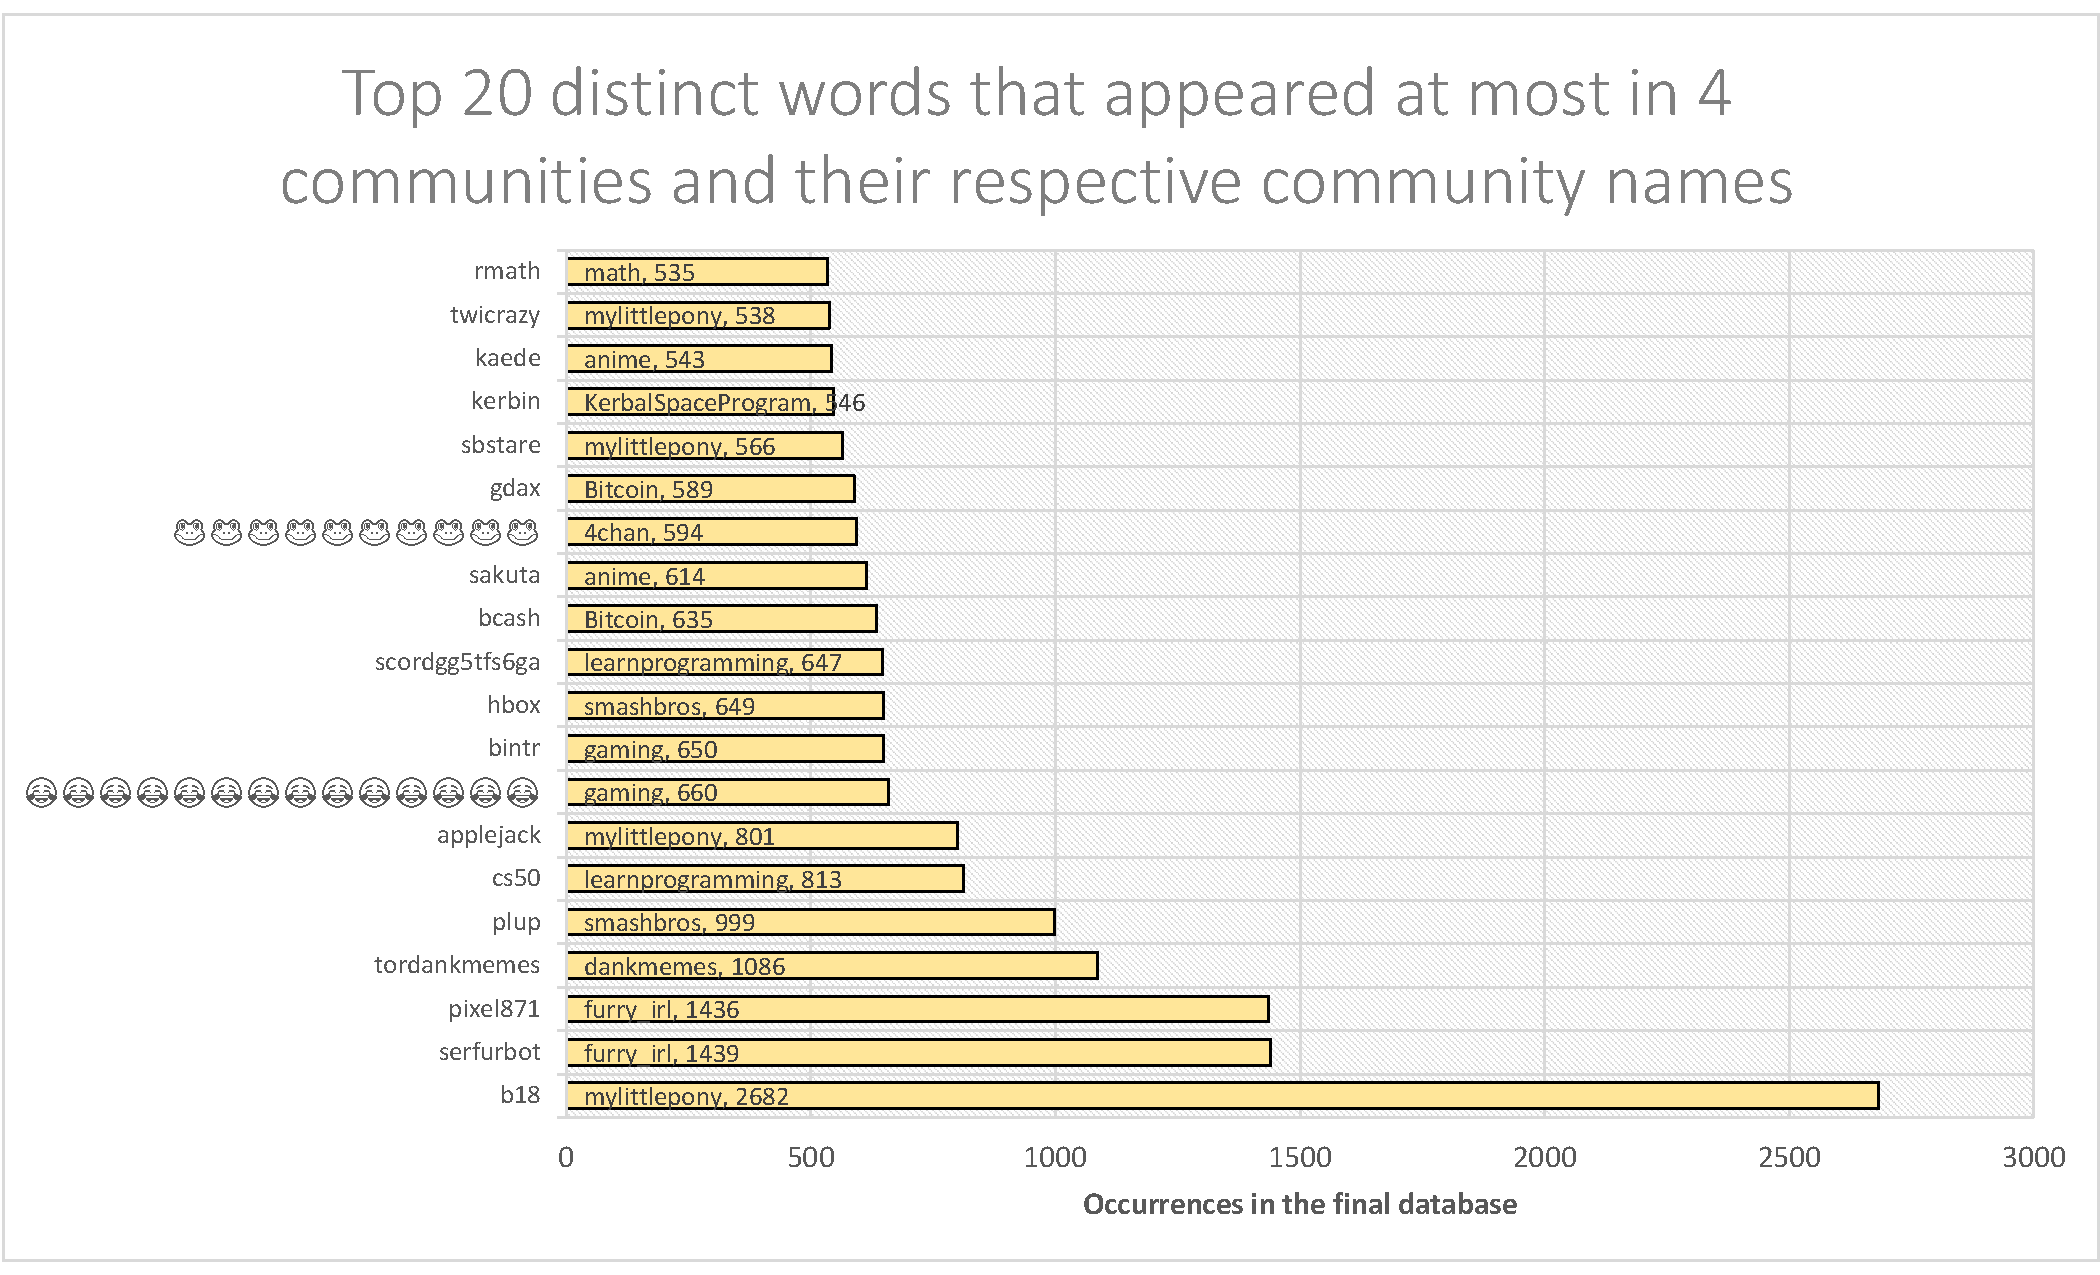
\includegraphics[width=\textwidth]{topdistinctwords.pdf}
    \caption{Twenty most distinct words with criteria specified above}
    \label{fig:mesh1}
\end{figure}


\subsubsection{Most common swear words}
By far, the most popular swear word in the database is "fuck", a word that does not necessarily condone negative emotions, it can be combined with positive emotions by saying things like "fuck yes". \\ \\
"shit", "damn", "hell" and "asshole" fill the remaining slots on the top five most popular swear words in the scraped database. \\ \\
Interestingly enough, the word "nigga" is more popular than the word "nigger". Though both of them are extremely offensive, the word "nigga" seems slightly softer than the word "nigger".\\ \\
The British word "arse" is only 4 times less popular than the American word "ass", but the word "asshole" is much, much more popular than the other two.
\begin{figure}[H]
    \centering
    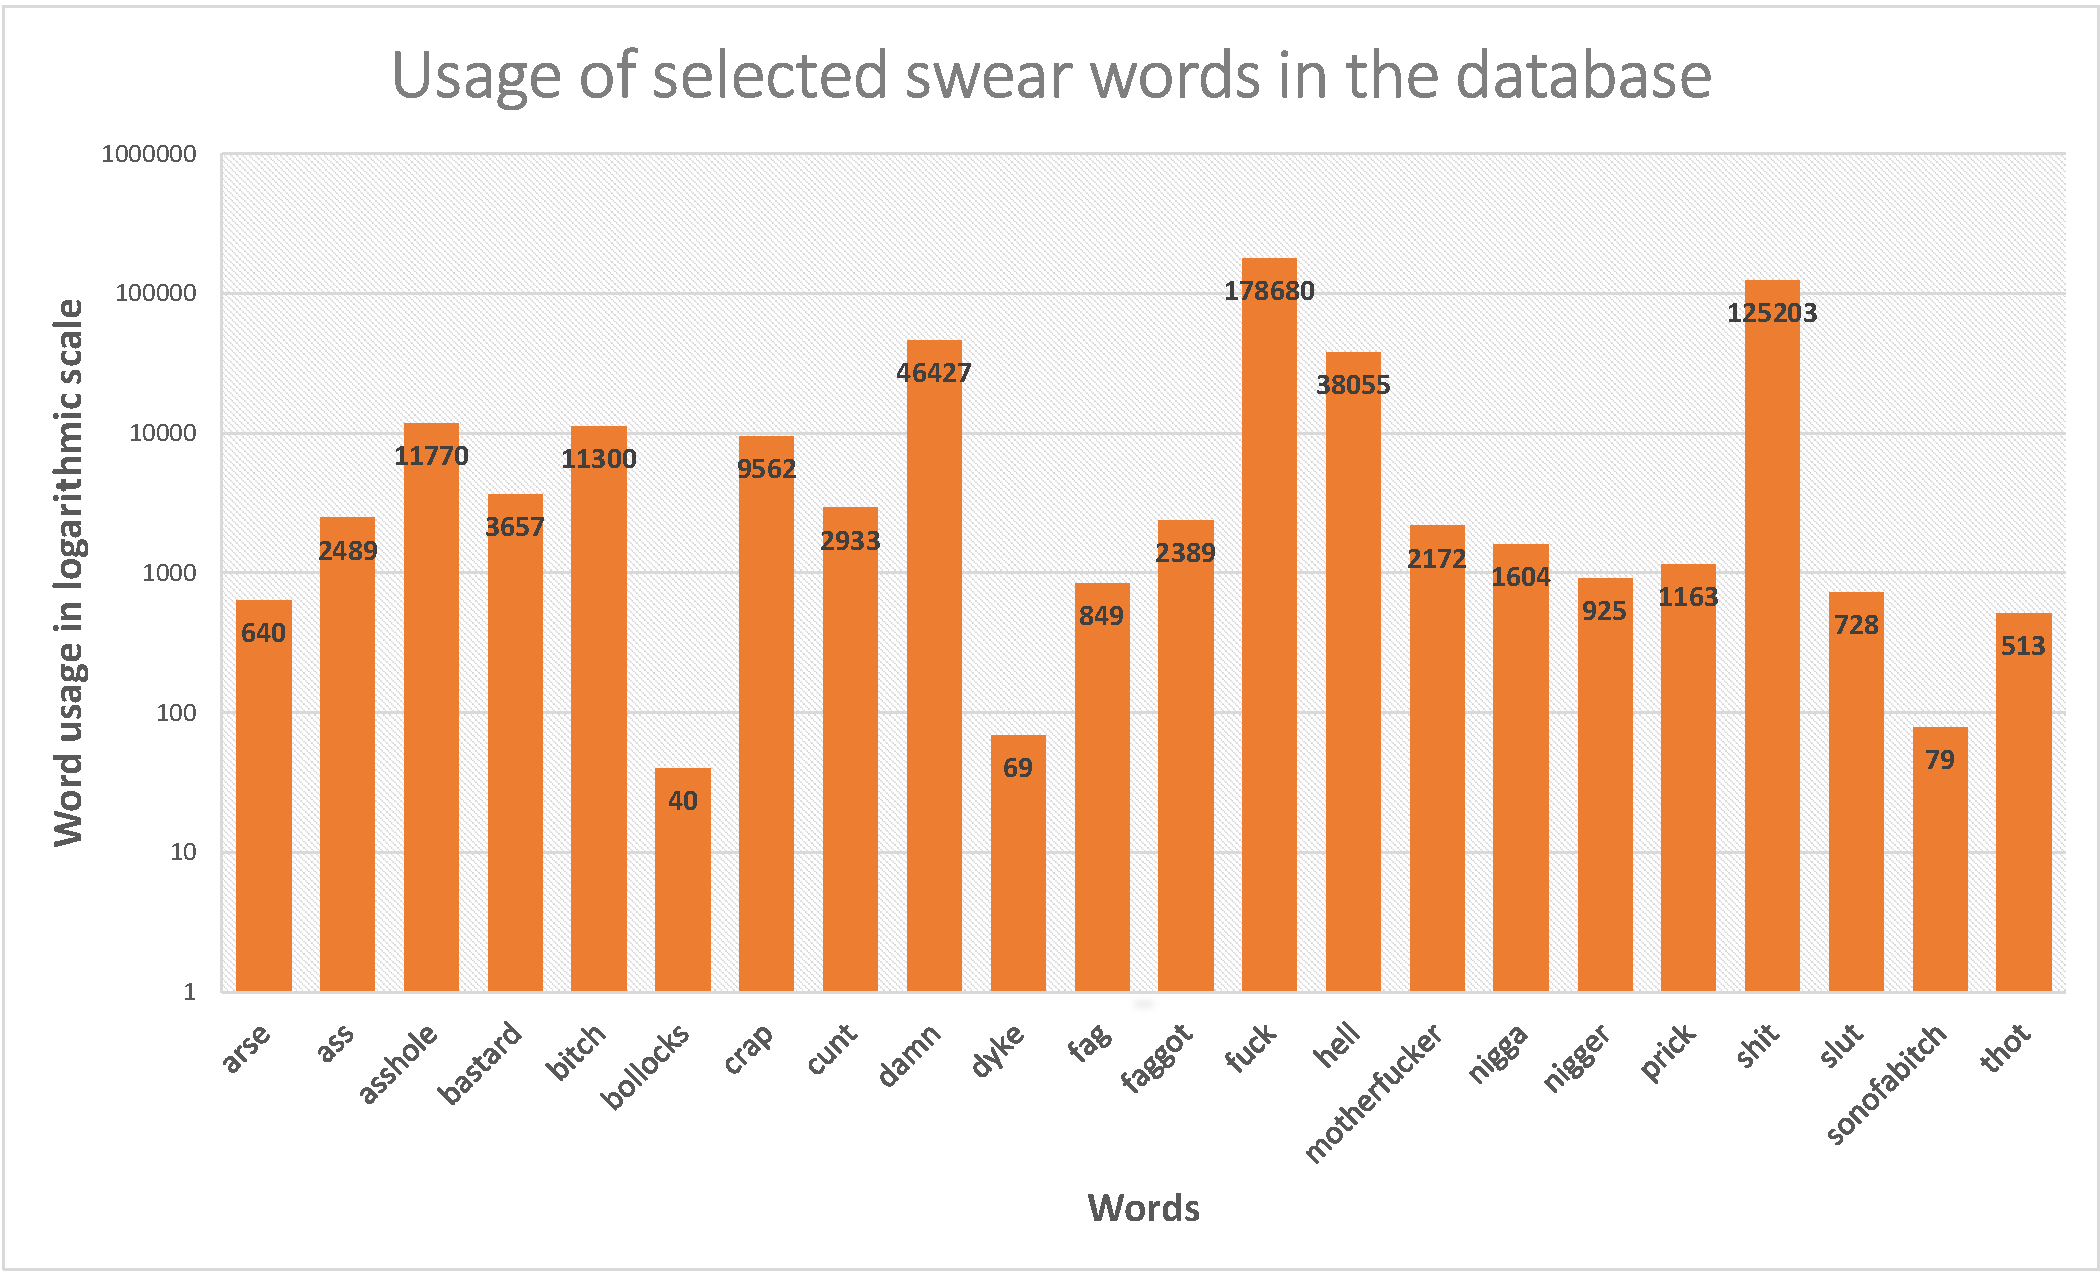
\includegraphics[width=\textwidth]{swearwords.pdf}
    \caption{List of the most popular swear words displayed in logarithmic scale}
    \label{fig:mesh1}
\end{figure}

\subsection{Positive and negative sentiment among Subreddits}
In order to determine whether posts on a Subreddit were positive or negative, IMDb reviews labeled "positive" and "negative" were utilized\cite{sentimentanalysis}. \\ \\
Comparing that trained dataset to our database led to the following conclusions:
\begin{itemize}
    \item Most of the Subreddits we have considered have had negative sentiment,
    \item Three of the most positive Subreddits are /r/gonewild (dedicated to NSFW photo posting), /r/itookapicture (dedicated to posting your own photos and getting constructive feedback) and /r/depression (most likely people in Comments kept giving themselves advice and reassuring themselves that things are going to get better),
    \item Three of the most negative Subreddits are /r/Drama (personal conflicts with other people), /r/mildlyinfuriating (people finding things to be annoyed about), and /r/4chan (a Subreddit dedicated to defy being politically correct),
    \item The most positive Subreddit is more positive than the most negative Subreddit is negative.
\end{itemize}
The data from this trial is visualized in the charts below.
\begin{figure}[H]
    \centering
    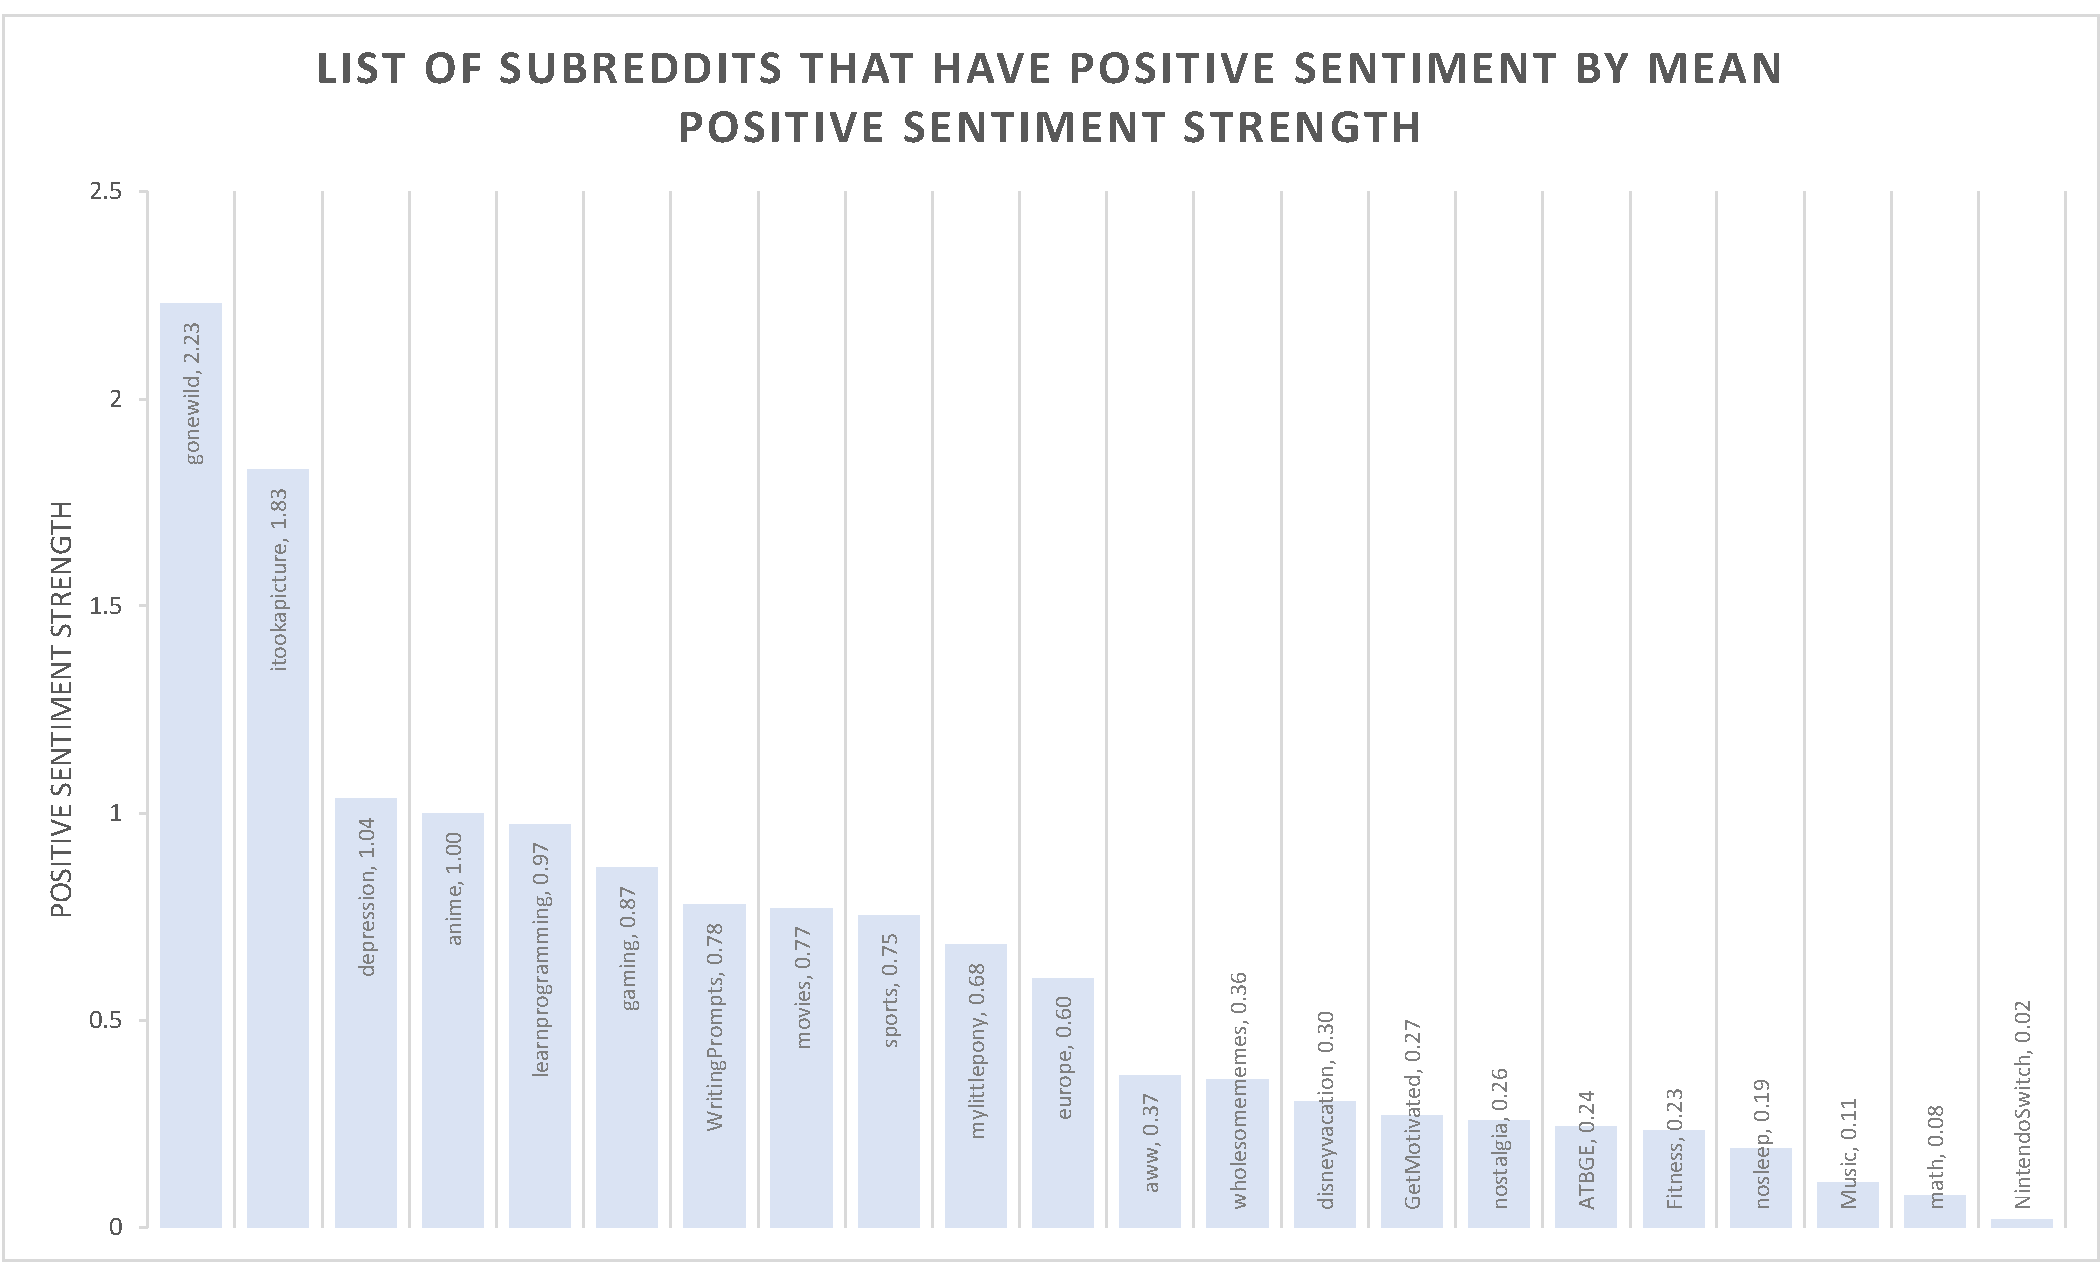
\includegraphics[width=\textwidth]{positivesentiment.pdf}
    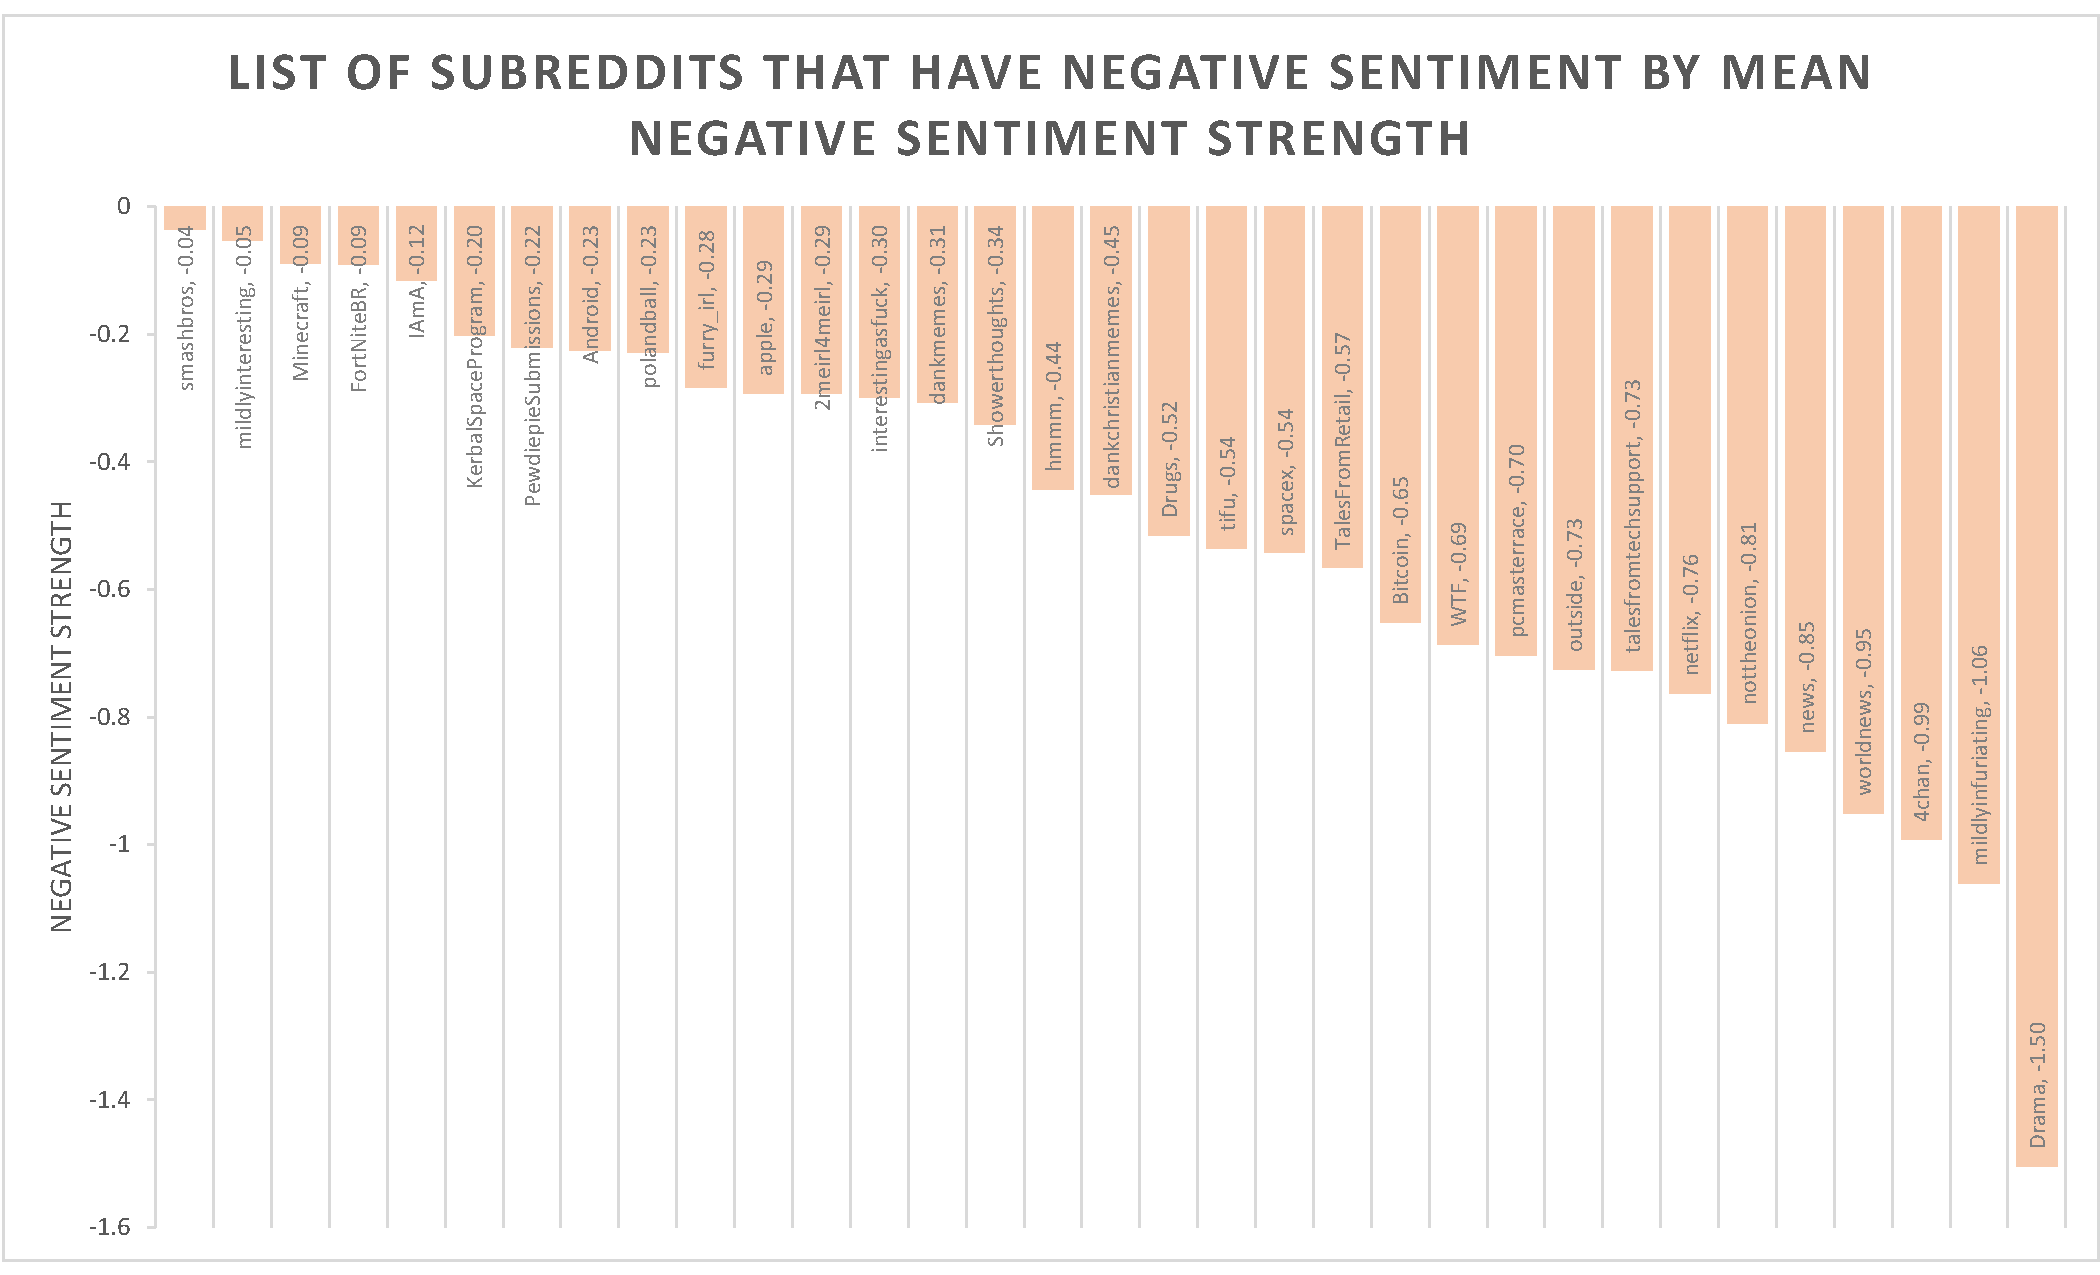
\includegraphics[width=\textwidth]{negativesentiment.pdf}
    \caption{Lists of Subreddits categorized by positive and negative sentiments}
    \label{fig:mesh1}
\end{figure}

\subsection{Selected n-grams}
The tool for n-grams allowed deriving n-gram .csv tables, which could be converted into charts.

\subsubsection{What does Reddit dream about}
By creating 4-grams containing input words of "want to" we can find out what are the dreams and ambitions of Reddit users.
\begin{figure}[H]
    \centering
    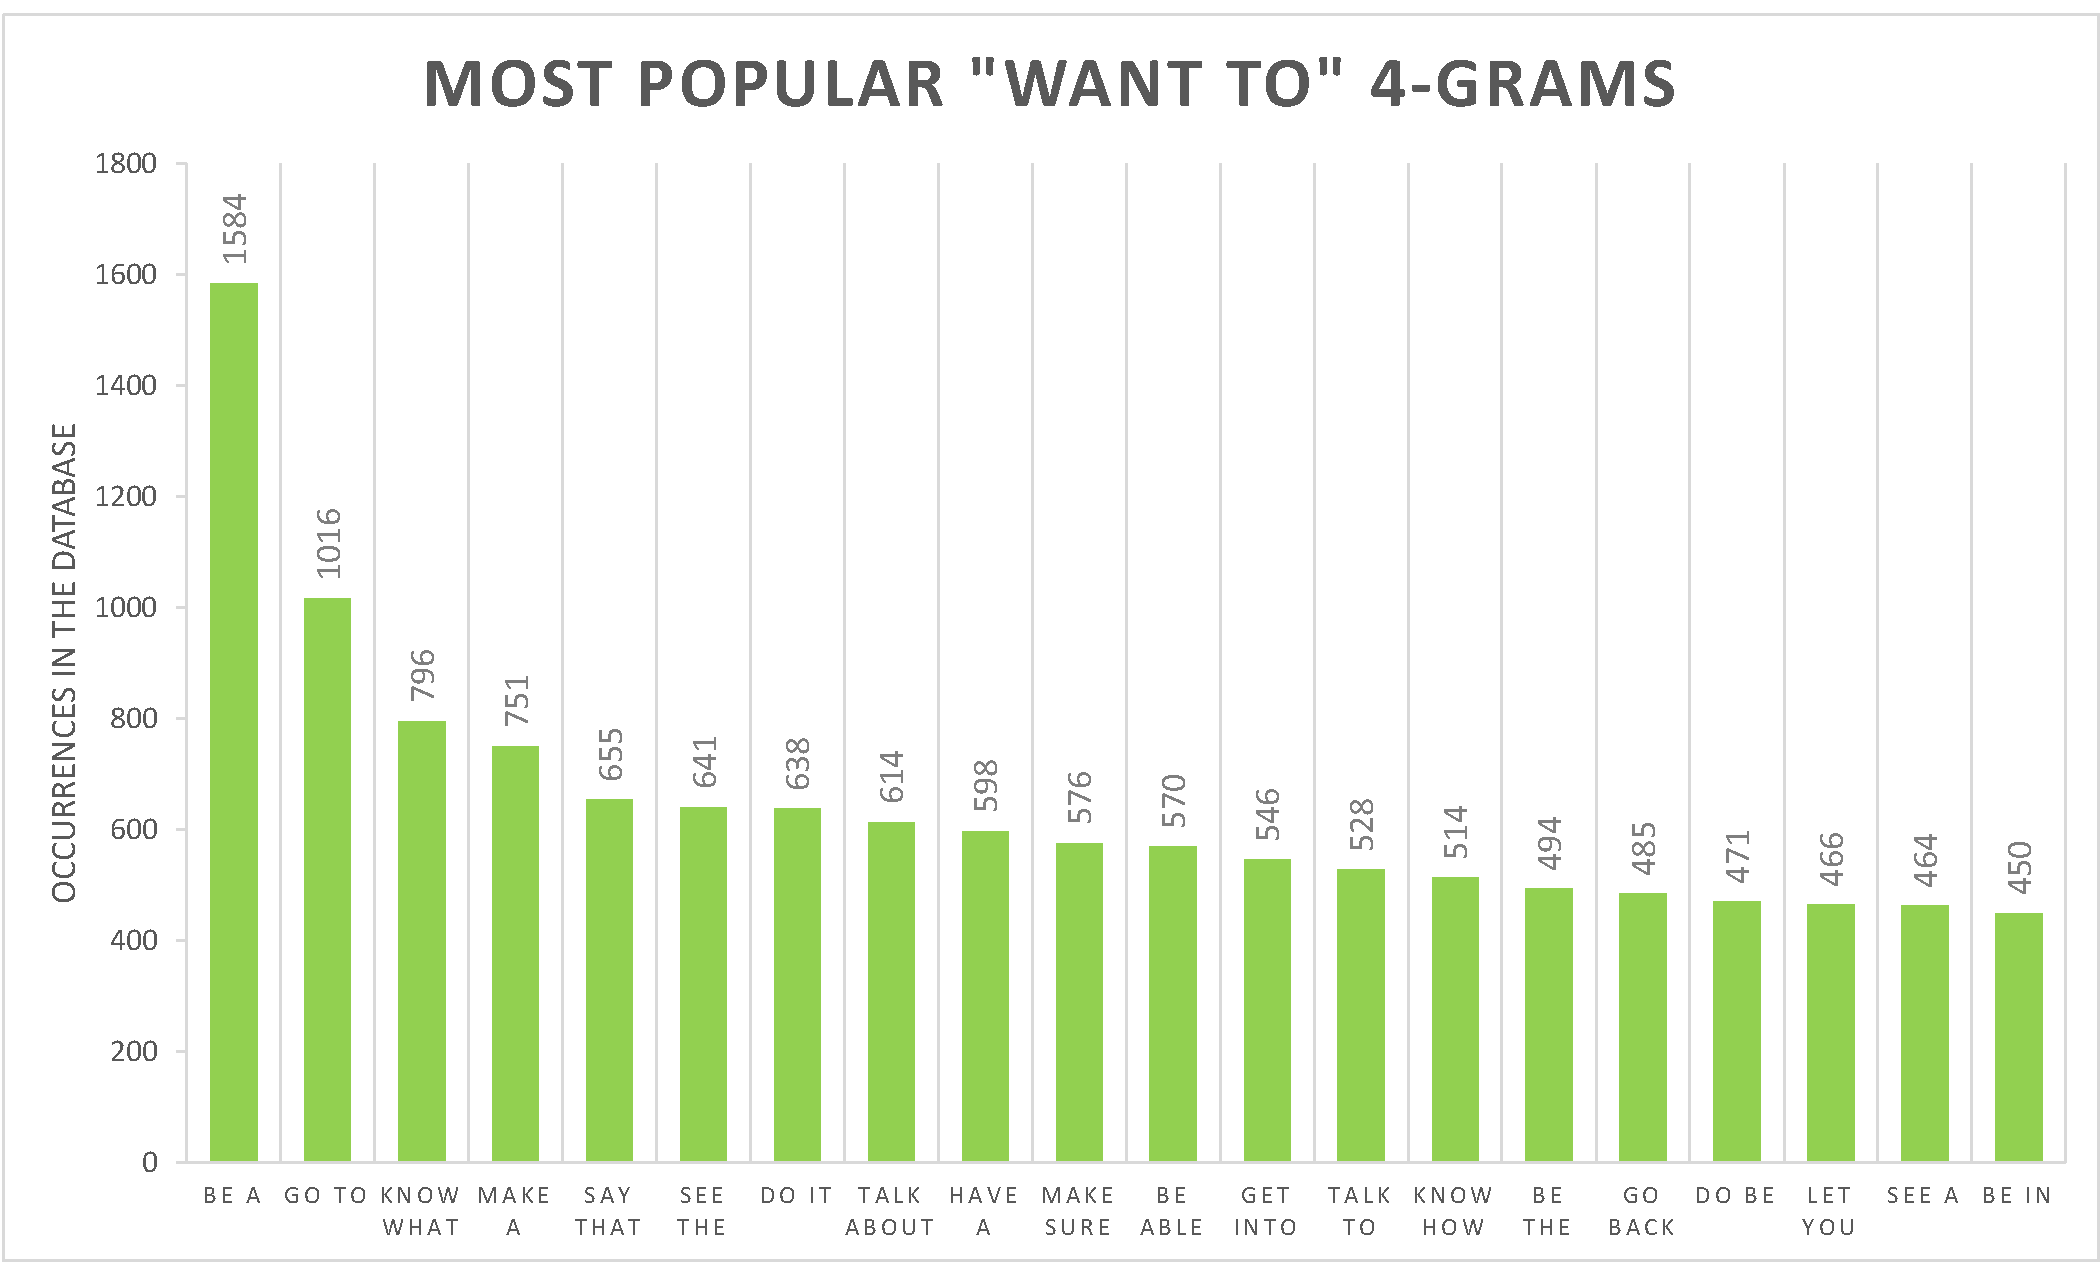
\includegraphics[width=\textwidth]{wantto.pdf}
    \caption{List of 4-grams starting with the phrase "want to"}
    \label{fig:mesh1}
\end{figure}
It seems as if most of the dreams of Reddit users concern their own experiences and working on self-improvement. The most common 4-grams, "want to be a", "want to go to", "want to know what" all seem to be related to self-improvement process. \\ \\
More altruistic phrases, "want to make sure", "want to talk to", "want to let you" trail behind the most common 4-grams, but their presence is still tangible in the database. \\ \\
The most common dreams seem to either become someone else, travel, discuss things with others or reassure that everything is still fine.

\subsubsection{Feelings}
To test what Reddit users are feeling, a search for 2-grams containing the word "feel" has been conducted. Surprisingly enough, the amount of positive and negative emotions in the database is pretty similar to one another.\\ \\
The most common word completing this 2-gram was the word "like", with the word "bad" being the fourth most common entry and the word "well" being the fifth one.

\begin{figure}[H]
    \centering
    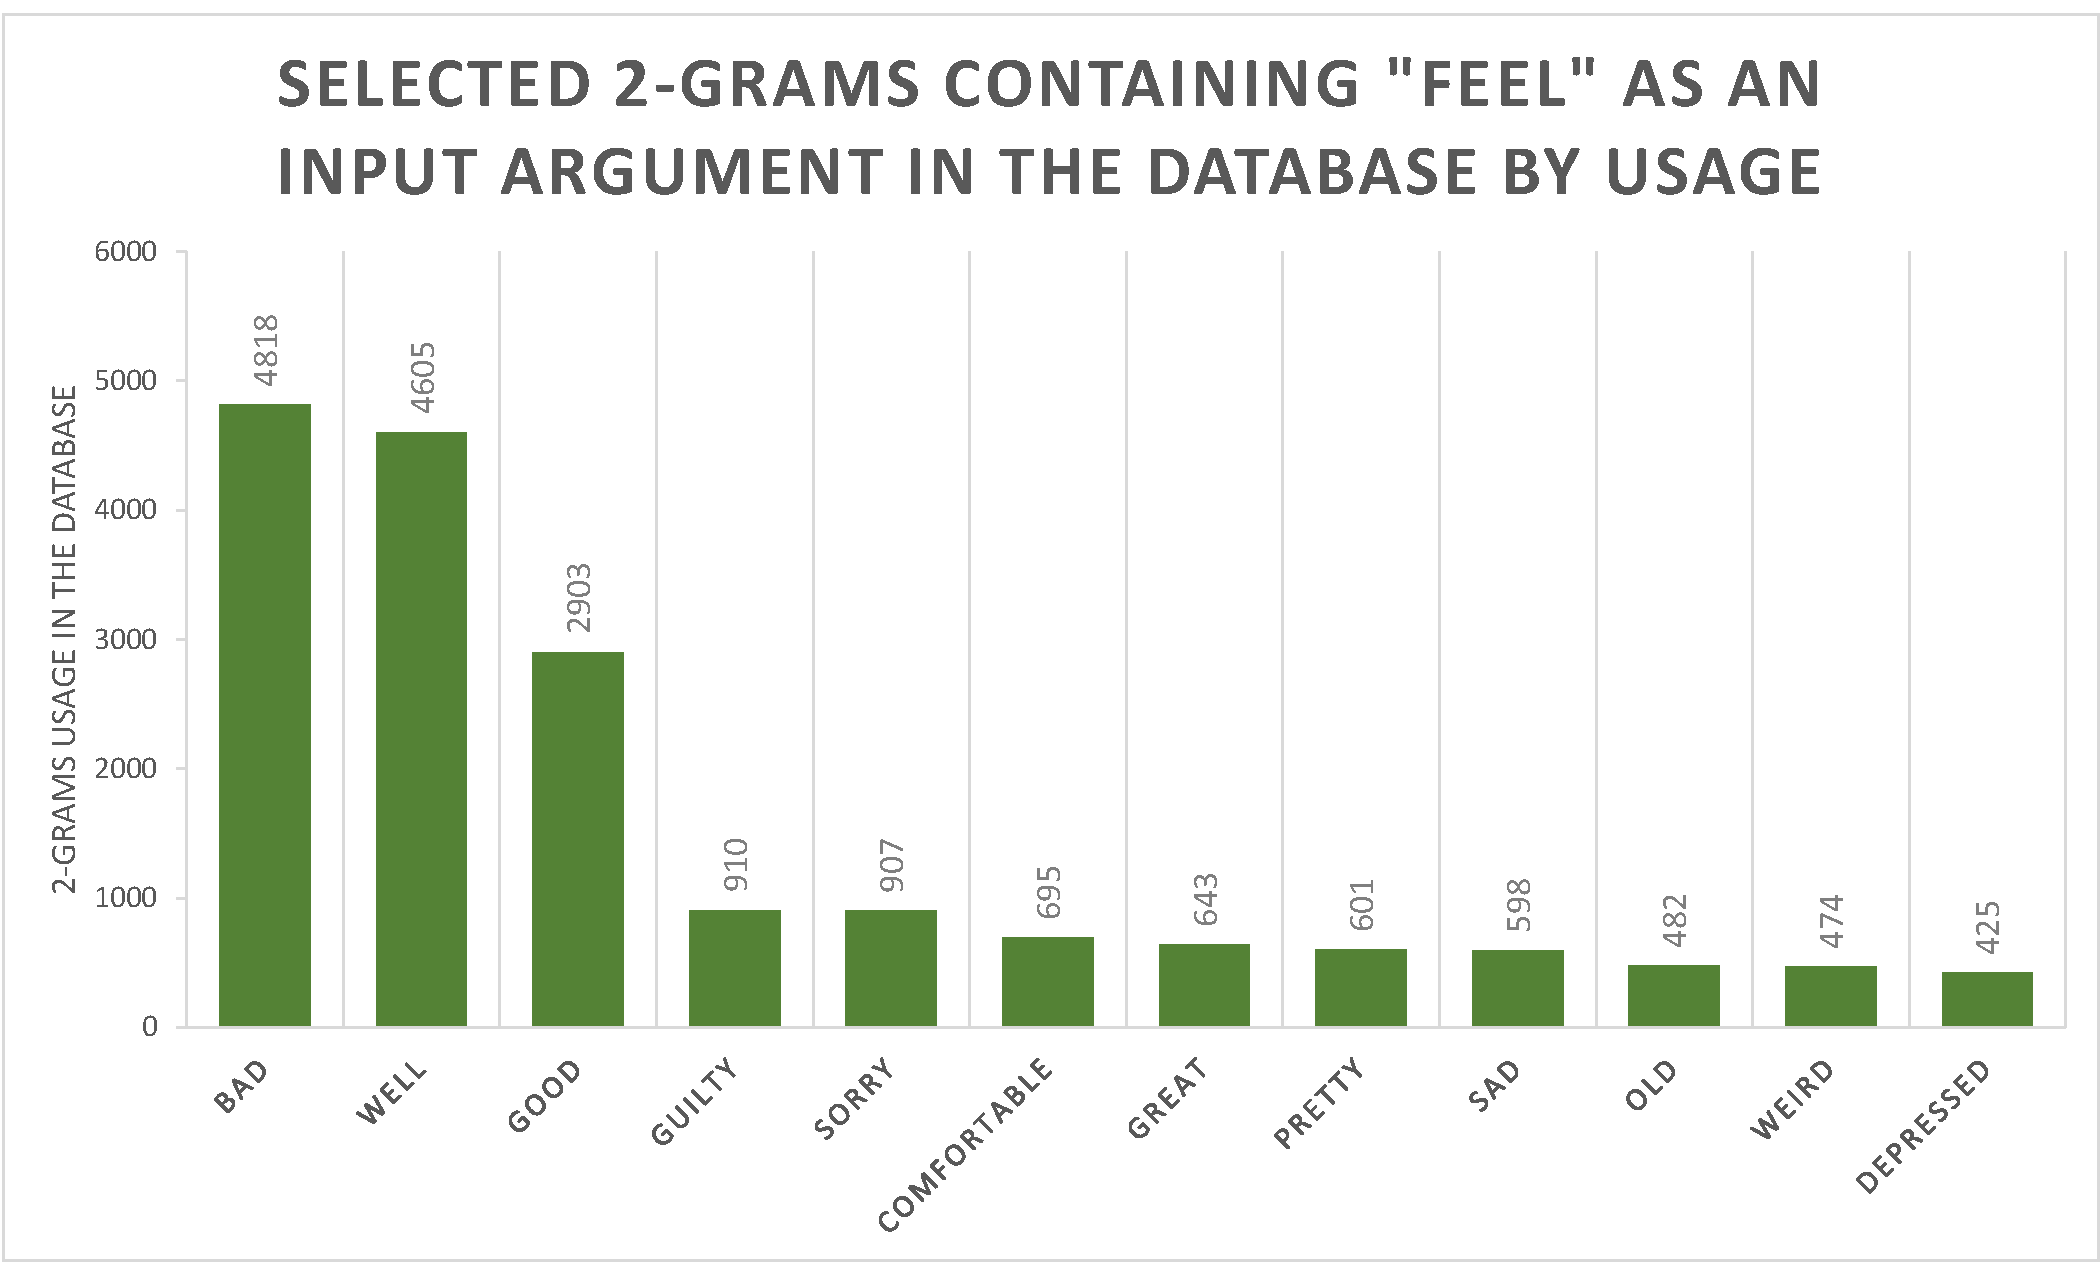
\includegraphics[width=\textwidth]{feel.pdf}
    \caption{List of 2-grams starting with the phrase "feel"}
    \label{fig:mesh1}
\end{figure}

\section{Post-mortem}
As it turns out, running scripts on Big Data takes very long time. In our project we have decided to consider Python as our main scripting language, which made it easier to run advanced scripts, but because of that the execution of scripts was very long.\\ \\
A major help in the process of statistic deriving were the statistics files containing  \href{https://drive.google.com/file/d/1_bkH21F-ifAVhdobl4DU-Rr_UDUYsjm0/view?usp=sharing}{most common words} in Subreddits created by Kamil Czerniak and an \href{https://drive.google.com/drive/folders/1izGHyl-19wRL2TkJFYoMKktoBgXTJ6yb}{average usage of words} .csv file arranged by Samuel Menezes, which later laid foundations to the work of three more people.

\subsection{What worked}
A huge, tremendous amount of data laid foundation to interesting statistics, creating comprehensive classifiers and interesting data tables. Everyone involved contributed to the project a fair share and laid the foundation for something that each of us can be proud of, that sits in the repository signed under our names and we can show off the data as projects we have participated in in our resumes.\\ \\
Every section of this document contains sweat and tears of people trying to pave the way onto the next members of this project.\\ \\
A huge part of the database survived the process of normalization and markdown removal, making place for a lot of data processing that helped create this final report.\\ \\
A few tools were created in the process of this project, all of them have made it much easier to process large amounts of data and interact with the database.

\subsection{What was learned}
A major part of the project was coded exclusively in Python. Because of that, the members that did not bite into Python before and those that have only briefly tried Python before, had to learn the basics of this language in order to run efficient scripts.\\ \\
A list of concepts relating to Natural Language Processing that was learned through the process of working on this project involves: tokenization, classification, lemmization, stop words, nltk corpuses, data tables, n-grams, data processing and the likes of it. \\ \\
If not for the Google Colab rental computing power, the project would not be in this position. The process of cleaning up the database ran on multiple different instances through an entire weekend trying to clean up the database.

\subsection{What didn't work}
Unfortunately, data from 4 Subreddits was lost in the process of cleaning up the database. Some of the most distinct words, like "pewdiepie" still show up as the most distinct to the Subreddit "/r/pewdiepiesubmissions", but less distinct words are no longer attributed to those four Subreddits. \\ \\
Being concise has proven itself to be a bigger challenge than expected. Though initially the responsibilities of some people were assigned for 2 weeks in advance, even having the work started a week before a deadline made people deliver either incomplete or wrong solutions. Often the goals of the project would be misunderstood or the scale of them miscalculated and they would have to be corrected over the following days.\\ \\
The part of the database containing NER labels has never been utilized, despite that some other Machine Learning (though pre-trained models) have found their way into the project\cite{sentimentanalysis}\cite{emotions}\cite{wordnet}.\\ \\
Because of how long Python scripts ran on the database, several stats have never made their way to the final report.

\subsection{Bonus materials}
Not every statistic made its way into the final document here, a special folder on Google Drive\cite{bonusmaterials} was made for all the .csv files that have been generated, but have not made their final way into this document. All the bonus files are available in that directory.

\addcontentsline{toc}{section}{References}
\begin{thebibliography}{xx}

\bibitem{stopwords}
Stop words in English language and the process of their removal\\
\href{https://www.geeksforgeeks.org/removing-stop-words-nltk-python/}{https://www.geeksforgeeks.org/removing-stop-words-nltk-python/}

\bibitem{sentimentanalysis} 
IMDb Sentiment NLP database used for sentiment analysis \\
\href{https://medium.com/@GeneAshis/nlp-sentiment-analysis-on-imdb-movie-dataset-fb0c4d346d23}{https://medium.com/@GeneAshis/nlp-sentiment-analysis-on-imdb-movie-dataset-fb0c4d346d23}

\bibitem{emotions}
Classification of Emotions into Valence, Arousal and Dominance\\
\href{https://saifmohammad.com/WebPages/nrc-vad.html}{https://saifmohammad.com/WebPages/nrc-vad.html}

\bibitem{wordnet}
Wordnet based Categorization Dictionary\\
\href{https://provalisresearch.com/products/content-analysis-software/wordstat-dictionary/wordnet-based-categorization-dictionary/}{https://provalisresearch.com/products/content-analysis-software/wordstat-dictionary/wordnet-based-categorization-dictionary/}

\bibitem{bonusmaterials}
Bonus .csv files created by us on Google Drive\\
\href{https://drive.google.com/drive/folders/1VMXW1Nha9ULm5C9VruYI4l-aEdbzAXXU?usp=sharing}{https://drive.google.com/drive/folders/1VMXW1Nha9ULm5C9VruYI4l-aEdbzAXXU?usp=sharing}

\end{thebibliography}


\end{document}
